\documentclass{thesisclass}
% Based on thesisclass.cls of Timo Rohrberg, 2009
% ----------------------------------------------------------------
% Thesis - Main document
% ----------------------------------------------------------------


%% -------------------------------
%% |  Information for PDF file   |
%% -------------------------------
\hypersetup{
 pdfauthor={Not set},
 pdftitle={Not set},
 pdfsubject={Not set},
 pdfkeywords={Not set}
}



%% ---------------------------------
%% | Information about the thesis  |
%% ---------------------------------

\newcommand{\myname}{thomas}
\newcommand{\mytitle}{Titel der Ausarbeitung bzw. des Themas}
\newcommand{\myinstitute}{Institut für Visualisierung und Datenanalyse,\\ Lehrstuhl für Computergrafik}

\newcommand{\reviewerone}{?}
\newcommand{\reviewertwo}{?}
\newcommand{\advisor}{?}
\newcommand{\advisortwo}{?}

\newcommand{\timestart}{XX. Monat 20XX}
\newcommand{\timeend}{XX. Monat 20XX}
\newcommand{\submissiontime}{DD. MM. 20XX}


%% ---------------------------------
%% | ToDo Marker - only for draft! |
%% ---------------------------------
% Remove this section for final version!
\setlength{\marginparwidth}{20mm}

\newcommand{\margtodo}
{\marginpar{\textbf{\textcolor{red}{ToDo}}}{}}

\newcommand{\todo}[1]
{{\textbf{\textcolor{red}{(\margtodo{}#1)}}}{}}


%% --------------------------------
%% | Old Marker - only for draft! |
%% --------------------------------
% Remove this section for final version!
\newenvironment{deprecated}
{\begin{color}{gray}}
{\end{color}}


%% --------------------------------
%% | Settings for word separation |
%% --------------------------------
% Help for separation:
% In german package the following hints are additionally available:
% "- = Additional separation
% "| = Suppress ligation and possible separation (e.g. Schaf"|fell)
% "~ = Hyphenation without separation (e.g. bergauf und "~ab)
% "= = Hyphenation with separation before and after
% "" = Separation without a hyphenation (e.g. und/""oder)

% Describe separation hints here:
\hyphenation{
% Pro-to-koll-in-stan-zen
% Ma-na-ge-ment  Netz-werk-ele-men-ten
% Netz-werk Netz-werk-re-ser-vie-rung
% Netz-werk-adap-ter Fein-ju-stier-ung
% Da-ten-strom-spe-zi-fi-ka-tion Pa-ket-rumpf
% Kon-troll-in-stanz
}


%% ------------------------
%% |    Including files   |
%% ------------------------
% Only files listed here will be included!
% Userful command for partially translating the document (for bug-fixing e.g.)
\includeonly{%
titlepage,
content
}


%%%%%%%%%%%%%%%%%%%%%%%%%%%%%%%%%
%% Here, main documents begins %%
%%%%%%%%%%%%%%%%%%%%%%%%%%%%%%%%%
\begin{document}

\nocite{*}

% Remove the following line for German text
%\selectlanguage{ngerman}

\frontmatter
\pagenumbering{roman}
%% titlepage.tex
%%

% coordinates for the bg shape on the titlepage
\newcommand{\diameter}{20}
\newcommand{\xone}{-15}
\newcommand{\xtwo}{160}
\newcommand{\yone}{15}
\newcommand{\ytwo}{-253}

\begin{titlepage}
% bg shape
\begin{tikzpicture}[overlay]
\draw[color=gray]  
 		 (\xone mm, \yone mm)
  -- (\xtwo mm, \yone mm)
 arc (90:0:\diameter pt) 
  -- (\xtwo mm + \diameter pt , \ytwo mm) 
	-- (\xone mm + \diameter pt , \ytwo mm)
 arc (270:180:\diameter pt)
	-- (\xone mm, \yone mm);
\end{tikzpicture}
	\begin{textblock}{10}[0,0](4,2.5)
		
\includegraphics[width=.3\textwidth]{logos/KITLogo_RGB.pdf}
	\end{textblock}
	\changefont{phv}{m}{n}	% helvetica	
	\vspace*{3.5cm}
	\begin{center}
		\Huge{\mytitle}
		\vspace*{2cm}\\
		\Large{
			Proseminar-Ausarbeitung von
		}\\
		\vspace*{1cm}
		\huge{\myname}\\
		\vspace*{1cm}
		\Large{
			An der Fakult\"at f\"ur Informatik
			\\
			\myinstitute
		}\\
		\vspace*{1cm}
		\Large{\today}
	\end{center}
	\vspace*{1cm}
%\Large{
%\begin{center}
%\begin{tabular}[ht]{l c l}
%  % Gutachter sind die Professoren, die die Arbeit bewerten. 
%  \iflanguage{english}{Reviewer}{Erstgutachter}: & \hfill  & \reviewerone\\
%  \iflanguage{english}{Second reviewer}{Zweitgutachter}: & \hfill  & \reviewertwo\\
%  \iflanguage{english}{Advisor}{Betreuender Mitarbeiter}: & \hfill  & \advisor\\
%  \iflanguage{english}{Second advisor}{Zweiter betreuender Mitarbeiter}: & \hfill  & \advisortwo\\
%  % Der zweite betreuende Mitarbeiter kann weggelassen werden. 
%\end{tabular}
%\end{center}
%}


\vspace{2cm}


\begin{textblock}{10}[0,0](4,16.8)
\tiny{ 
		{KIT -- Universität des Landes Baden-Württemberg und nationales Forschungszentrum der Helmholtz-Gesellschaft}
}
\end{textblock}

\begin{textblock}{10}[0,0](14,16.75)
\large{
	\textbf{www.kit.edu} 
}
\end{textblock}

\end{titlepage}

\blankpage


%% -------------------
%% |   Directories   |
%% -------------------
\tableofcontents
\blankpage


%% -----------------
%% |   Main part   |
%% -----------------
\mainmatter
\pagenumbering{arabic}
%% content.tex
%%

%% Einleitung.tex
%% $Id: einleitung.tex 28 2007-01-18 16:31:32Z bless $
%%

\chapter{Einleitung}
\label{ch:Einleitung}
%% ==============================
Hinweis: In die Einleitung gehört die Motivation 
und Einleitung in die Problemstellung. Die Problemstellung
kann in der Analyse noch detaillierter beschrieben werden.


%% ==============================
\section{Zielsetzung der Arbeit}
%% ==============================
\label{ch:Einleitung:sec:Zielsetzung}

Was ist die Aufgabe der Arbeit? \ldots

%% Zielsetzung der Arbeit.tex
%% $Id: Zielsetzung der Arbeit.tex 28 2007-01-18 16:31:32Z bless $
%%

Jedes Jahr werden neue Smartphones ver{\"o}ffentlicht und vorgegaukelt das alles neu entwickelt wurde. Dabei {\"a}ndern sich nur die inneren Komponenten durch einen neuen Prozessor und kleinen Softwareupdates sowie eine minimale Verbesserung an der Kamera. 
Es wird immer davon gesprochen, dass man dem Benutzer mit dem neuen Smartphone ein besseres Erlebnis bieten m{\"o}chte. 


Durch diese Abhandlung widmet sich die Frage, wie weit kann ein Smartphone individuell personalisiert werden. 
%Dabei stellt man die Frage, wie weit kann man ein Smartphone so personalisieren, dass es genau f{\"u}r eine Person angepasst ist? 
Unter den Standardeinstellungen kann man zwar ein Hintergrundbild, einzelne Klingelt{\"o}ne, Schriftgr{\"o}{\ss}en und die Platzierungen der Apps anpassen. 
Aber das ist alles nur f{\"u}r die visuellen sowie audiovisuellen Wahrnehmungen. 
Wie soll man unterschiedliche Informationen wahrnehmen, wenn das Smartphone auf dem Tisch oder in der Hosentasche ist und das Smartphone auf stumm gestellt ist? 

Aus diesem Grund verfolge man das Ziel, personalisierte Vibrationssignale mittels dem vorgegebenen Wearable zu erstellen.
%Im Rahmen dieser Bachelorarbeit verfolge man das Ziel, personalisierte Vibrationssignale zu erstellen.
Hierbei werden drei verschiedene Vibrationssignale f{\"u}r einen Nutzer so angepasst, dass die Werte speziell f{\"u}r den Benutzer bestimmt werden. 
Zur Bestimmung der Vibrationssignale wird ein Evolution{\"a}rer Algorithmus verwendet. Nachdem diese Handlungsvorschrift die passenden Werte gefunden hat, wird {\"u}berpr{\"u}ft, wie gut die Benutzer die personalisierten Vibrationssignale im Vergleich zu vorgegebenen Werten erkennen können.
%wie gut die personalisierten Vibrationssignale im Vergleich zu vorgegebenen Werten erkannt werden. 
Es hat sich dabei die Hypothese gebildet, dass die personalisierten Vibrationen besser erkannt werden als die vorgegebenen Vibrationen.

%Die Aufgabe besteht darin, f{\"u}r ein Individuum mit einem Programm drei verschiedene Vibrationssignale f{\"u}r Ihn so anzupassen, dass die Werte von Ihm besser erkannt werden als vorgegebene Werte. Dabei wird zur Bestimmung eines Vibrationssignals ein Evolution{\"a}rer Algorithmus verwendet. Nachdem dieser passende Wert gefunden worden ist, wird {\"u}berpr{\"u}ft, wie gut im Vergleich zu vorgegebenen Werten die Daten erkannt werden.

%Somit wollte man herausfinden, ob es m{\"o}glich ist f{\"u}r jedes Individuum eine eigene passende L{\"a}nge und St{\"a}rke von Vibrationssignalen zu erstellen, sodass die Kombination der Signale noch erkannt werden.

%Die Hypothese, die man mit dieser Bachelorarbeit beantworten m{\"o}chte ist, ob man mittels personalisierten Vibrationen eine Folge von Vibrationen besser unterscheiden als vorgegebene Vibrationen.
%Um dies beantworten zu k{\"o}nnen verwende man ein Wearable zur Darstellung der Vibrationssignale und den Evolution{\"a}ren Algorithmus um die personalisierten Vibrationen zu ermitteln.



%% ==============================
\section{Gliederung der Arbeit}
%% ==============================
\label{ch:Einleitung:sec:Gliederung}

Was enthalten die weiteren Kapitel? \ldots

%% Gliederung der Arbeit.tex
%% $Id: GliederungDerArbeit.tex 28 2007-01-18 16:31:32Z bless $
%%

Im Verlauf dieser Bachelorarbeit erläutere ich erst allgemein, was die einzelnen Bestandteile des Evolutionären Algorithmus sind und wie ich den an mein Problem angepasst habe. Sowie das Problem ansatzweise heutzutage umgesetzt wurde und wie ich an das Problem heranging und wie ich es Implementiert haben.

// auskommentieren
In meiner Bachelorarbeit werde ich erst einmal erläutern, was aktuell in den Smartphones und in der Forschung benutzt wird.
Im Folgenden werde ich erläutern, was ein Genetischer Algorithmus ist und wie ich diesen nutze genutzt habe. 

%%% Local Variables: 
%%% mode: latex
%%% TeX-master: "diplarb"
%%% End: 


%% grundlagen.tex
%% $Id: grundlagen.tex 28 2007-01-18 16:31:32Z bless $
%%

\chapter{Grundlagen}
\label{ch:Grundlagen}
%% ==============================
%Die Grundlagen müssen soweit beschrieben
%werden, dass ein Leser das Problem und
%die Probleml{\"o}sung  versteht.Um nicht zuviel 
%zu beschreiben, kann man das auch erst gegen 
%Ende der Arbeit schreiben.

%Bla fasel\ldots

%% ==============================
\section{Taktile Ger{\"a}te}
%% ==============================
\label{ch:Grundlagen:sec:Taktile Ger{\"a}te}



%% taktile ger{\"a}ate.tex
%% $Id: taktilegeraete.tex 28 2007-01-18 16:31:32Z bless $
%%

Ein Taktiles Ger{\"a}t ist ein Ger{\"a}t, dass Informationen an einen Menschen durch die Wahrnehmung der Haut mitteilt.\cite{gemperle2001design}
% mitteilen m{\"o}chte, dies geschieht durch die Wahrnehmung der Haut. 

Taktile Ger{\"a}te werden heutzutage {\"o}fter verwendet, als man es eigentlich wahrnimmt. 
Ein einfaches Beispiel ist das Smartphone. 
Eine Person trägt sein eigenes Smartphone in der Hosentasche. 
Bei einer eingehenden Nachricht, muss der Benutzer mitgeteilt werden, dass eine Nachricht empfangen wurde.
Normalerweise geschieht das beim Abspielen des Klingeltons. Falls man besch{\"a}ftigt ist und nicht durch ein lautes Klingeln gest{\"o}rt werden will, stellt man den Ton ab. 
Um dennoch den Nutzer darauf Aufmerksam zu machen, dass eine Nachricht eingetroffen ist, wird die Vibration des Smartphones verwendet.
%spielt die Vibration des Smartphones eine große Rolle. 
%verwendet man die Vibration des Smartphones.
%Um dennoch darauf Aufmerksam zu machen, dass eine Nachricht eingetroffen ist, nutzt man die Vibration des Smartphones.

%Das Smartphone ist nur eins von vielen Beispielen, was man {\"u}ber den Alltag noch f{\"u}r Taktile Ger{\"a}te verwendet.
Ein weiteres Beispiel in der Taktile Displays benutzt werden ist f{\"u}r Blinde Menschen, um Wissen zu {\"u}bermitteln \cite{parente2003bats}. 
F{\"u}r Blinde gibt es spezielle Karten, die Konturen f{\"u}r die Umrisse der L{\"a}nder darstellen, solche Karten sind selten vertreten.
Um ein solches Ungleichgewicht zwischen den blinden und normal sehenden Sch{\"u}lern zu mindern, hat man sich ein System entwickelt, dass audiovisuelle und taktile Eindr{\"u}cke vereint. 
Dabei hat man sich f{\"u}r eines r{\"a}umlich akustisches Soundsystem entschieden, um den Sch{\"u}ler anhand Ger{\"a}uschen aus verschiedenen Richtungen ein Gef{\"u}hl zu geben, an welchen Orten man sich aktuell befindet und was um einen herum passiert. 
Es wurden nicht nur Tier- und Verkehrsger{\"a}usche verwendet, sondern auch den Namen der Region, in der man sich aktuell befindet, wurde ausgespeochen. 
Als Taktiles Device hat man sich an schon existierenden M{\"a}usen und Controllern bedient, die Force-Feedback besa{\ss}en. 

Die verwendeten Karten waren nicht so detailliert wie in der Realit{\"a}t.
%Die Karten, die man verwendet hat, sind nicht so detailliert, wie normale Karten. 
Im Vergleich zu der normalen Karten hat man hier weniger Informationen, die man {\"u}bertragen muss und die Details der L{\"a}ndergrenzen konnte man leichter darstellen. 

Damit ein Sch{\"u}ler eine Karte erkunden konnte, bewegt er sich mithilfe eines Eingabeger{\"a}ts {\"u}ber die Karte und dr{\"u}ckt eine Taste auf der Tastatur um Informationen {\"u}ber das Gebiet abzurufen, diese wurden {\"u}ber Audios {\"u}bermittelt. Das Taktile Device wurde verwendet um Grenz{\"u}berg{\"a}nge zu mittels Vibrationen zu signalisieren.





%% ==============================
\section{Evolution{\"a}rer Algorithmus}
%% ==============================
\label{ch:Grundlagen:sec:Genetischer Algorithmus}


%% Genetischer Algorithmus.tex
%% $Id: Genetischer Algorithmus.tex 28 2007-01-18 16:31:32Z bless $
%%

Die Evalutionären Algorithmen sind stochastische Optimierungsverfahren. Man findet damit nicht die beste Lösung für ein Problem, jedoch findet man eine gute Annäherung.
Dabei hat man sich bei den Evolutionären Algorithmen an der Biologischen Evolution von Darwin inspirieren lassen. \cite{selzam2003genetische}

In der Biologie ist jeder lebende Organismus ein Induvidiuum.
Jedes Induvidiuum besitzt Erbinformationen in der Form von Chromosomen. Die Erbinformationen werden auch \textbf{Gene} oder \textbf{DNA} genannt.
Eine Gruppe von Induviduen wird als \textbf{Population} bezeichnet.

Der Algorithmus wurde anhand der folgenden Merkmale erstellt.

%% ==============================
\subsection{Selektion}
%% ==============================
\label{ch:Grundlagen:sec:Taktile Geräte:subsec:Selektion}

Eine \textbf{Selektion} ist ein Mechanismus, bei dem man sich zwei Individuen auswählt, um anschließend die Gene der beiden Individuen, mittels der sogenannten \textbf{Rekombination}, zu kombinieren. Dabei gibt es verschiedene Selektionsstrategien. Man versucht die Individuen zu finden, um eine bestmöglichste Lösung für ein Problem zu liefern.

%% ==============================
\subsection{Variation}
%% ==============================
\label{ch:Grundlagen:sec:Taktile Geräte:subsec:Variation}

Man sollte eine zahlreiche Variation von Genen der einzelnen Individuen besitzen. 
Denn nehme anhand einem Beispiel von Süßigkeiten einmal kurz an, dass alle Süßigkeiten die gleiche Farbe und die gleiche Form haben. Wenn man sich jetzt zwei zufällige Süßigkeiten auswählen würde, hätten Sie keinerlei unterschiede und so würde das Nachkommen die gleichen Gene besitzen. Damit genau das nicht auftaucht, versucht man zu Beginn eine große Variation an Individuen zu erzeugen und diese als Anfangs Population für einen Evolutionären Algorithmus zu nutzen. Mittels Rekombination und Mutation wird dabei ein neues Induvidiuum für die nächste Generation erzeugt. 


//Durch Rekombination und Mutation der DNA der Induviduuen erhält man eine Variation. 
//Die Rekombination und Mutation erzeugt lediglich ein neues Induviduum aus der DNA der zuvor selektierten Induviduen.

Um die nächsten Generationen zu bilden wird eine Rekombination und Mutation auf die DNA der Selektierten Induviduen ausgeführt. 
Die Variation der DNA  spielt eine wichtige Rolle, denn die ist für die nachfolgende Rekombination und Mutation entscheident für die nächsten Generationen. 
Um bei der Selektion unterschiedliche Induviduuen ausgewählt werden können, benötigt man zunächst eine Variation 

%% ==============================
\subsection{Vererbung / Gendrift}
%% ==============================
\label{ch:Grundlagen:sec:Taktile Geräte:subsec:Variation}
Bla fasel \dots

%% ==============================
\subsection{Allgeimeiner Vorgang eines Evolutionären Algorithmus}
%% ==============================
\label{ch:Grundlagen:sec:Taktile Geräte:sec:Allgeimeiner Vorgang eines Evolutionären Algorithmus}
Ein Evolutionärer Algorithmus besitzt grundsätzlich immer die gleichen Komponenten die miteinander.

%% ==============================
\subsection{Initialisierung}
%% ==============================
\label{ch:Grundlagen:sec:Initialisierung}
Man erzeugt sich zur Initialisierung eine Population von Individuen, die eine Variation von Genen besitzt. 

%% ==============================
\subsection{Bewertung der Individuen}
%% ==============================
\label{ch:Grundlagen:sec:Bewertung der Individuen}
Bevor man eine neue Population für die nächste Generation berechnen kann, muss man zuerst mithilfe einer Fitnessfunktion jedes Induvidiuum einen Fitnesswert bestimmen. 

%% ==============================
\subsection{Selektion}
%% ==============================
\label{ch:Grundlagen:sec:Selektion}
Anhand dem Fitnesswert der Induviduen werden zwei zufällige Induviduen bestimmt. Diese selektierten Induviduen werden als Eltern für die Nächste Generation benutzt.
Bei der Selektion wird ein hoher Fitnesswert bevorzugt.

%% ==============================
\subsection{Rekombination}
%% ==============================
\label{ch:Grundlagen:sec:Rekombination}
Die Gene der ausgewählten Eltern werden miteinander kombiniert und bilden die Gene des neuen Induvidiuum für die Population der nächsten Generation. Hier gibt es verschiedene Kombinationsmöglichkeiten, die angewendet werden können.

%% ==============================
\subsection{Mutation}
%% ==============================
\label{ch:Grundlagen:sec:Mutation}
Bei dem erzeugen Induvidiuum besteht eine Chance, dass die kombinierten Gene durch eine Mutation verändert werden. 

%% ==============================
\subsection{Wiederholung durch neuer Generation}
%% ==============================
\label{ch:Grundlagen:sec:Wiederholung durch neuer Generation}
Der Vorgang der Selektion, Rekombination und Mutation wird so oft ausgeführt, bis man eine neue Population hat, die genauso groß ist, wie die Anfangapopulation.
Nachdem die neue Population erzeugt wurde, wird diese durch die Anfangspopulation ersetzt und man führt den Algorithmus erneut aus. 
Dies geschieht so lange, bis man eine hinreichende Lösung für das Problem hat. 




Ich habe meinen Evolutionären Algorithmus so angepasst, dass bei mir ein Induviduum ein Signal ist. 
Ich habe dem Benutzer das Signal mit dem Wearable abspielen lassen und im Anschluss Fragen beantworten lassen. 
Er sollte bewerten wie gut er das Signal erkannt hat. Die Bewertung vom Benutzer war entscheidend um nach der kompletten Bewertung der Population 

%% ==============================
\section{Verwandte Arbeiten}
%% ==============================
\label{ch:Grundlagen:sec:RelatedWork}
%Hier kommt "`Related Work"' rein.
%Eine Literaturrecherche sollte so vollst{\"a}ndig wie m{\"o}glich sein,
%relevante Ans{\"a}tze m{\"u}ssen beschrieben werden und es sollte deutlich 
%gemacht werden, wo diese Ans{\"a}tze Defizite aufweisen oder nicht
%anwendbar sind, z.\,B. weil sie von anderen Umgebungen oder 
%Voraussetzungen ausgehen.


%% custom vibs.tex
%% $Id: Genetischer Algorithmus.tex 28 2007-01-18 16:31:32Z bless $
%%

Da heutzutage beinahe jedes Ger{\"a}t ein Vibrationsmotor verbaut hat, sei es das Handy, die Smartwatches oder Fitnessarmb{\"a}nder (u.v.m.), werde ich im folgenden auf einige aktuelle Technologien und deren Umsetzung der personalisierten Vibrationsmuster zu sprechen kommen. 

%% ==============================
\subsection{Taptic Engine}
%% ==============================
\label{ch:Grundlagen:sec:RelatedWork:subsec:TapticEngine}

Die Taptic Engine ist ein von der Firma Apple selbst entwickeltes Vibrationsmotor, dass heutzutage in nahezu allen Apple Produkten verbaut ist. Das erste Ger{\"a}t, was die Taptic Engine bekommen hat, war die Apple Watch. Der Name \textbf{Taptic} bildet sich aus dem W{\"o}rtern "`Taktil"' und "`Haptisch"'. 
Trotz der neu Erfindung einer mechanischen R{\"u}ckmeldung, bietet Apple keine Personalisierung, wie lange eine R{\"u}ckmeldung f{\"u}r die Apple Watch erfolgen soll. Die Einstellungsm{\"o}glichkeiten an der Apple Watch ist lediglich die St{\"a}rke der Vibration. Diese ist in 3 St{\"a}rkestufen unterteilt. Meiner Ansicht nach kann man daher nicht wirklich von einer personalisierten Vibration sprechen. 

\begin{figure}[htbp] 
	\centering
	\begin{minipage}[t]{0.4\textwidth}
		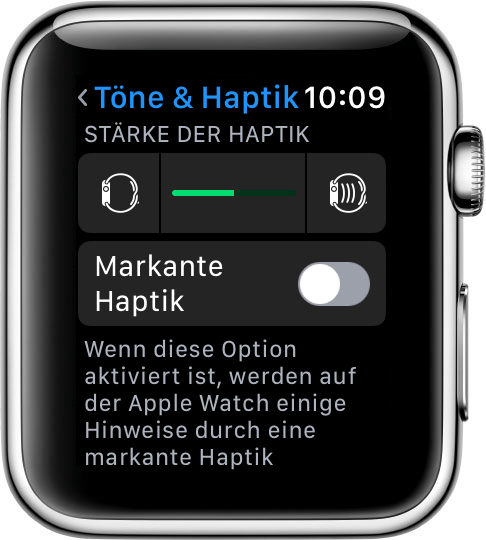
\includegraphics[width=\textwidth]{pics/applewatch.png}
	\end{minipage}
	\begin{minipage}[t]{0.4\textwidth}
		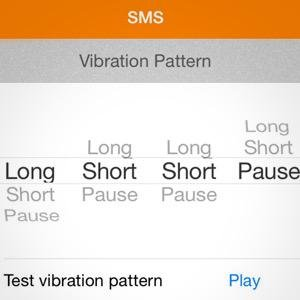
\includegraphics[width=\textwidth]{pics/martian.jpg}
	\end{minipage}
	\caption{Einstellungsm{\"o}glichkeit auf der Apple Watch (links) und in der Martian App (rechts)}
	\label{fig:Bild10}
\end{figure}

%\begin{figure}
%	\centering
%    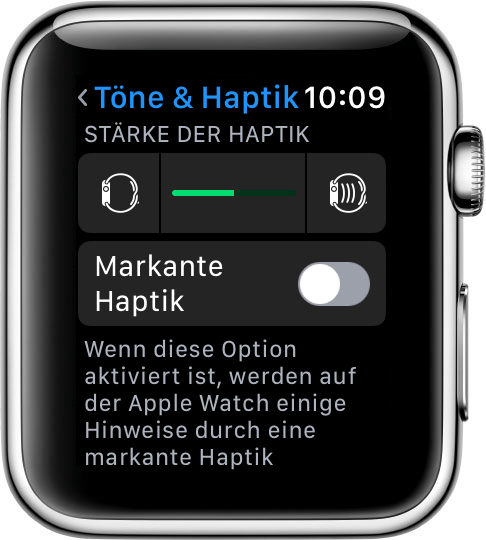
\includegraphics[width=\textwidth]{pics/applewatch.png}
%    \caption{Settings on the apple watch}
%    \label{fig:applewatch}
%\end{figure}
 
%% ==============================
\subsection{iPhone}
%% ==============================
\label{ch:Grundlagen:sec:RelatedWork:subsec:PersonalisierteVibration}

\begin{figure}
	\centering
    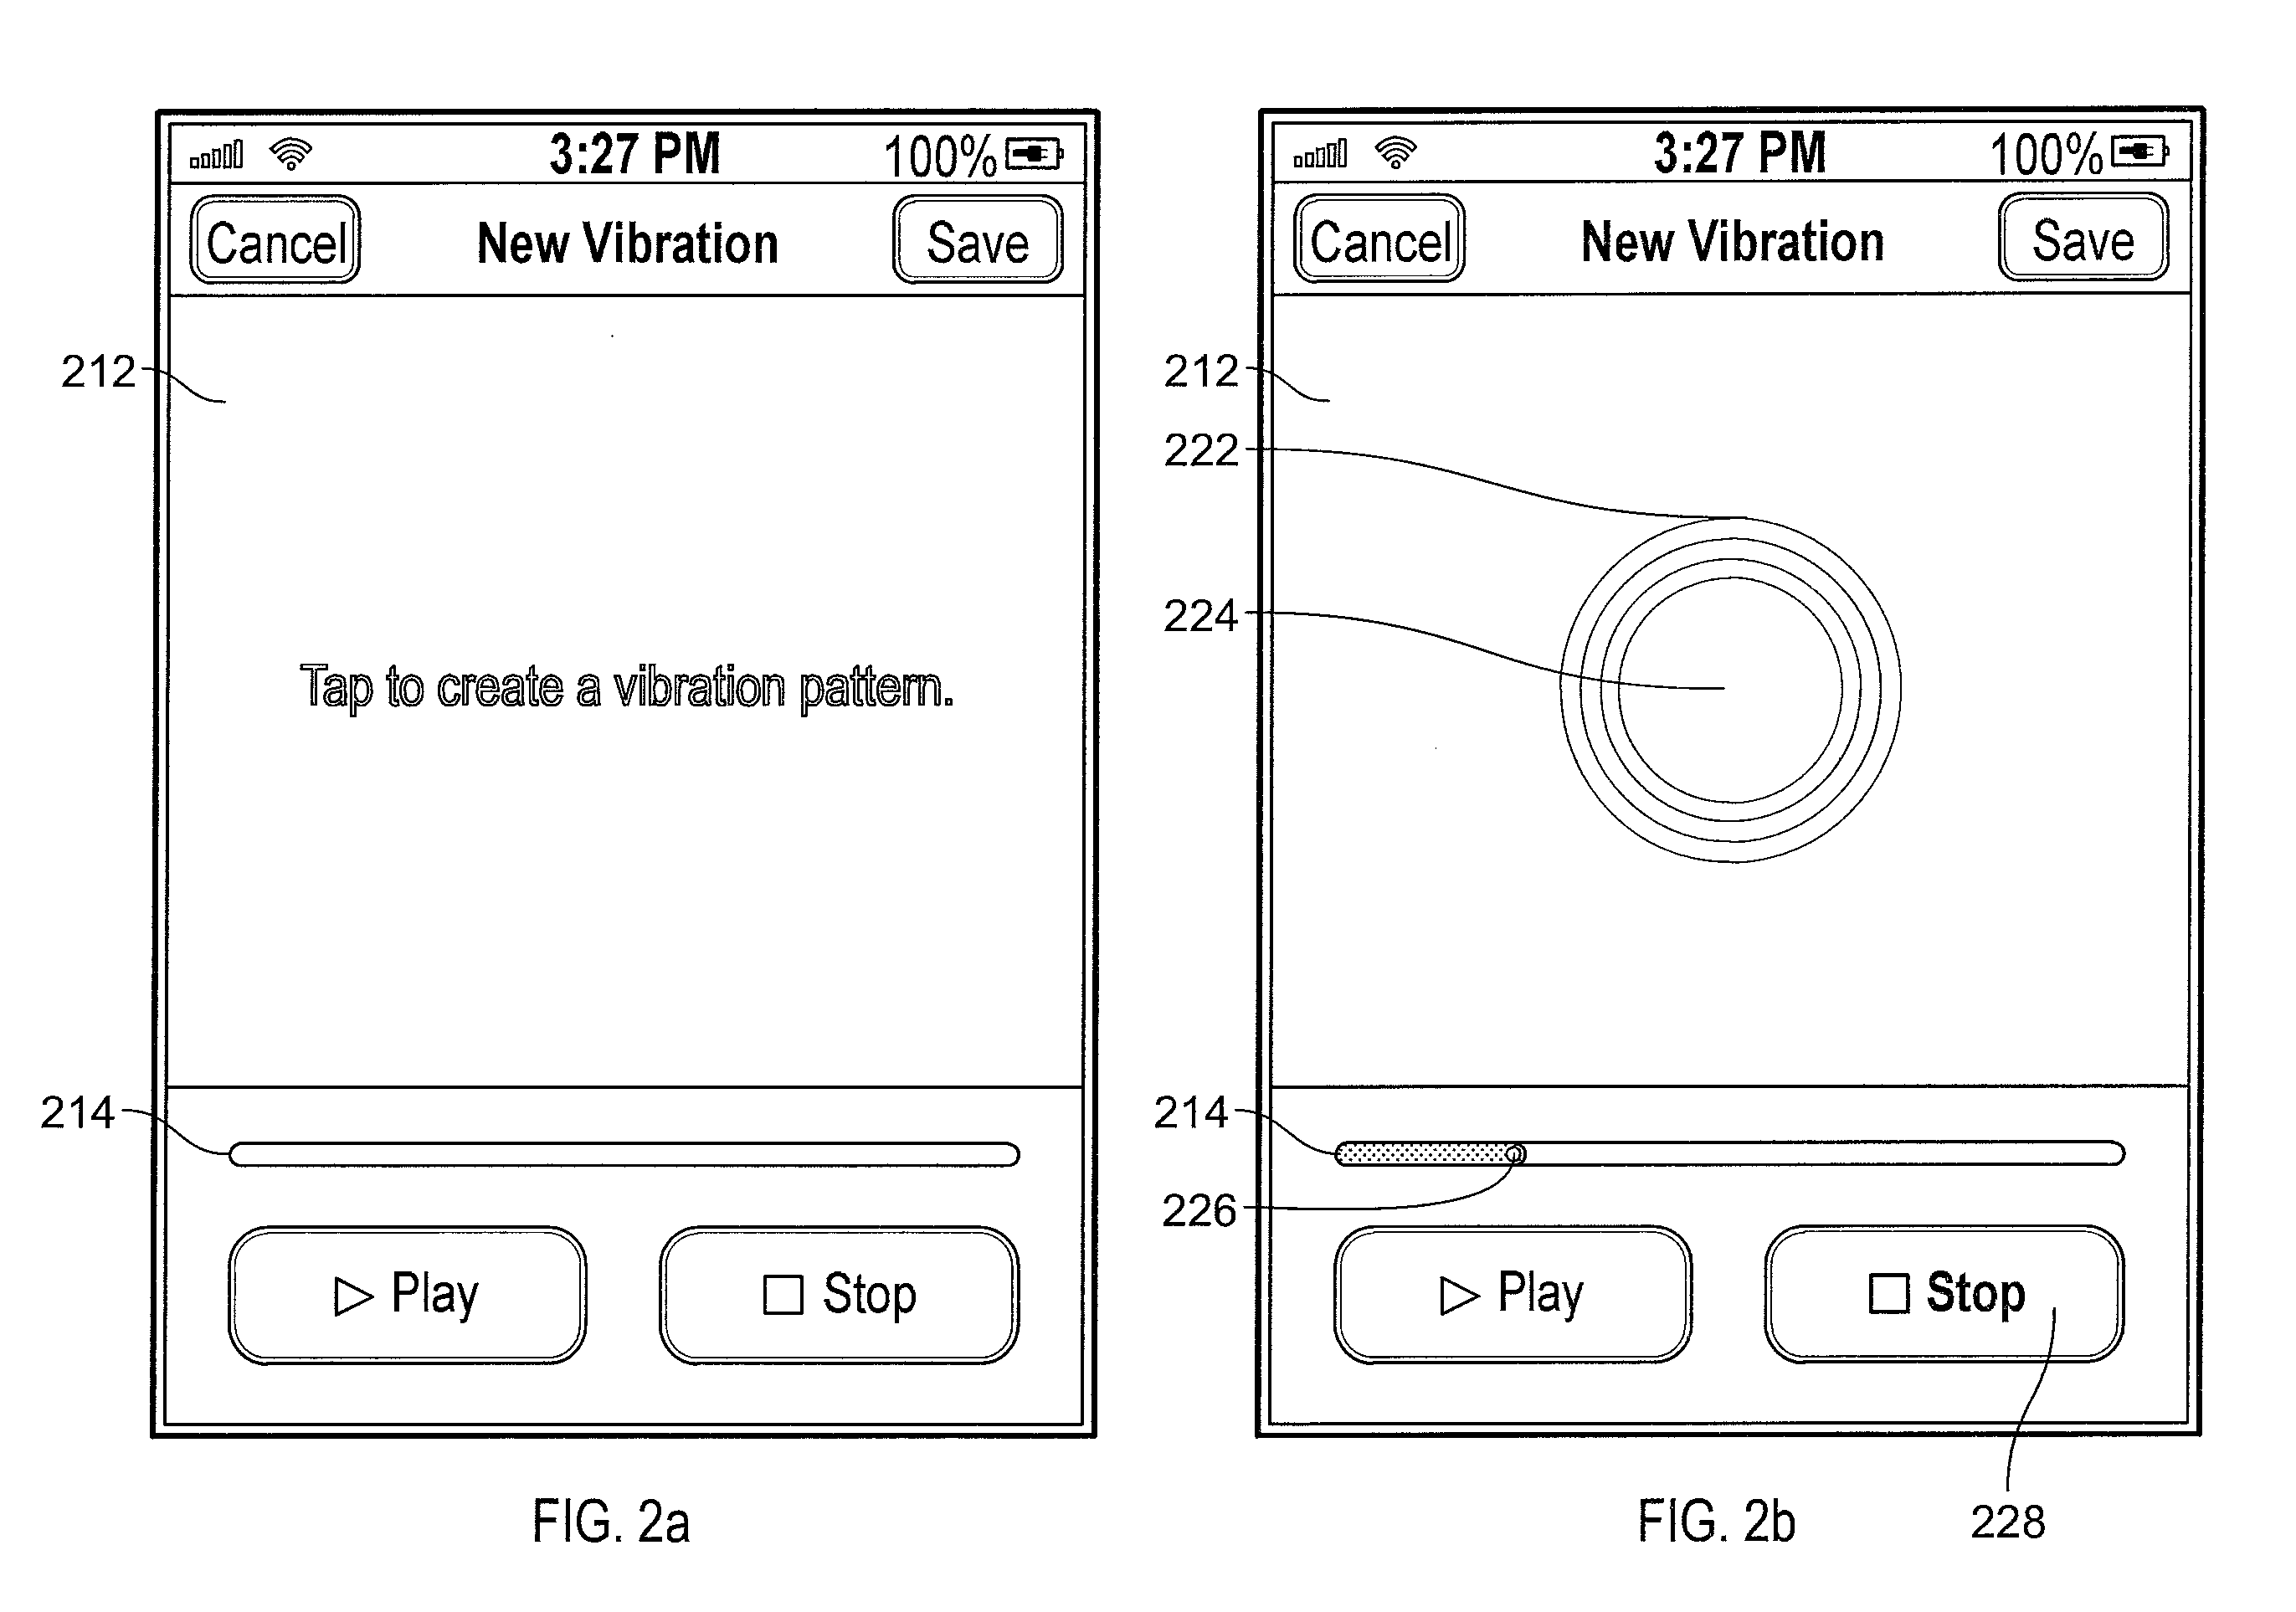
\includegraphics[width=\textwidth]{pics/iphone.png}
    \caption{Erstellung eigener Vibrationsmuster auf dem iPhone}
    \label{fig:iphone}
\end{figure}

Der Hersteller Apple hat auch bei dem iPhone eine M{\"o}glichkeit geboten, eigene Vibrationsmuster zu erstellen, jedoch mit Einschr{\"a}nkungen.
Wenn man in die jeweilige Einstellung der iPhones gelangt, erscheint das folgende Bild \autoref{fig:iphone}. 
Beim Dr{\"u}cken auf das Display wird an der Stelle eine Vibration erzeugt. 
Man hat 10 Sekunden um ein eigenes Muster zu erzeugen, indem man wiederholt auf den Bildschirm dr{\"u}ckt. 
An der Stelle, an der man den Bildschirm ber{\"u}hrt hat, erscheint visuell um der Position ein Kreis. 
Die erzeugten Vibrationen werden in einer Leiste visuell angezeigt. 
Man kann sich beliebig viele Vibrationsmuster speichern, die bis zu 10 Sekunden lang sind. \cite{fleizach2016custom}

Die Einschr{\"a}nkung, die man hier erw{\"a}hnen muss ist, dass man die Vibrationsmuster nur f{\"u}r Systeminterne Funktionen benutzen kann. 
Dies bedeutet, dass man die Funktionen f{\"u}r Klingelt{\"o}ne, Nachrichtent{\"o}ne, Erinnerungshinweise, Kalenderhinweise (o. {\"a}.) hinzuf{\"u}gen kann. 
F{\"u}r eine andere Anwendung, die nicht im Betriebssystem integriert sind, ist das nicht m{\"o}glich. 
Somit k{\"o}nnen Benachrichtigungen von anderen Entwicklern keine eigenen Vibrationsmuster erhalten. 
Tr{\"a}gt man das iPhone in der Hosentasche und es wird eine Benachrichtigung einer Applikation empfangen, die nicht im System integriert ist, kann man anhand der Vibrationen des iPhones nicht unterscheiden, welche Application dies gewesen ist.
%Daraus folgt, wenn das iPhone in der Hosentasche ist und ich eine Benachrichtigung von einer Application erhalte, die nicht im System integriert gewesen ist, kann man anhand der Vibrationen des iPhones nicht unterscheiden welche Application dies gewesen ist.
% kann man bei Benachrichtigungen von anderen Entwicklern nicht anhand der Vibrationen des iPhones  unterscheiden.

%% ==============================
\subsection{Martian Smartwatch}
%% ==============================
\label{ch:Grundlagen:sec:RelatedWork:subsec:PersonalisierteSmartwatch}

%\begin{figure}
%	\centering
%    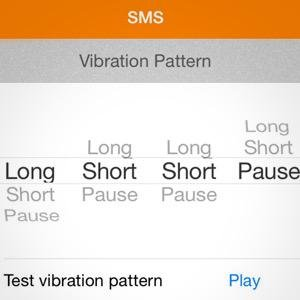
\includegraphics[width=\textwidth]{pics/martian.jpg}
%    \caption{possible settings on the martian watch}
%    \label{fig:martian}
%\end{figure}

Das Ger{\"a}t, das es nach meiner Recherche am besten gel{\"o}st hat, ist eine Smartwatch von einem kleinen Startup namens Martian. 
Das Startup hat eine Uhr hergestellt, mit der man mittels einer App auf dem Smartphone die Vibrationsmuster selbst anpassen kann. 
Die App unterst{\"u}tzt eine gro{\ss}e Anzahl an Applikationen, von anderen Herstellern, die Benachrichtigungen senden. 
Ein Vibrationsmuster f{\"u}r die Uhr kann man aus mit zu 4 Signalen auf der Uhr darstellen. 
Die Signale sind als Lang, Kurz und Pause festgelegt. 
Somit kann man mittels der Vibration der Uhr herausfinden, welche App gerade eine Benachrichtigung auf mein Handy gesendet hat. 
Die L{\"a}nge und St{\"a}rke eines Signals sind vom Hersteller festgelegt und kann nicht ge{\"a}ndert werden.

%% ==============================
\subsection{Andere Hersteller}
%% ==============================
\label{ch:Grundlagen:sec:RelatedWork:subsec:PersonalisierteSmartwatch}
Bei sehr vielen Herstellern ist es aktuell noch gar nicht m{\"o}glich eigene Vibrationsmuster zu erstellen. 
Bei Android Ger{\"a}ten ist es aktuell so, dass man aus einer Menge von wenigen vordefinierten Vibrationsmustern sich nur einen ausw{\"a}hlen kann. 
Einige Entwickler haben dieses Problem erkannt und eigene Applikationen entwickelt, die im Store ver{\"o}ffentlicht sind.







%% ==============================
\subsection{Design of a Wearable Tactile Displays}
%% ==============================
%% taktile geraeate paper.tex
%% $Id: taktilegeraetepaper.tex 28 2007-01-18 16:31:32Z bless $
%%

In dem Paper von \cite{gemperle2001design} handelt es um Taktile Displays; 
was man bei der Erschaffung von Taktilen Display beachten soll und was f{\"u}r Verwendungszwecke es noch gibt. 
Das Paper ist schon mehr als 15 Jahre alt und weist dennoch auf Informationen hin, die heutzutage noch Relevant sind. 
Die Inhalte des Papers werden im folgenden beschrieben.
Wie oben bereits erw{\"a}hnt wurde, sind Taktile Displays Ger{\"a}te, die dazu benutzt werden um Informationen durch K{\"o}rperkontakt des Menschen {\"u}ber Haptisches Feedback zu {\"u}bermitteln. Diese bilden keinen Konflikt mit den audio-/visuellen Einfl{\"u}ssen. 
Die Taktilen Displays sind eine Unterst{\"u}tzung der Darstellung der Informationen. 
Beispielsweise kann man Blinden oder Tauben Informationen mittels Taktilen Displays vermitteln, die Sie nicht wahrnehmen k{\"o}nnen.
Dabei werden haptische / sensorische assistive Ger{\"a}te benutzt um die Informationen aus der realen Umgebung in taktile Simulationen umzuwandeln.
Ein wichtiger Aspekt in diesem Paper ist es gewesen, wie man ein solches Taktiles Display entwirft.
Au{\ss}erdem gibt es Aspekte die man beim Entwurf beachten sollte:
%Au{\ss}erdem gibt es Aspekte die man beim Entwurf beachten sollte, wie Stromverbrauch zu reduzieren; leise, leicht und klein sein; sowie das die Taktoren durch die Kleidung sp{\"u}rbar ist und am besten so eng wie m{\"o}glich am K{\"o}rper liegt.
\begin{itemize}
\item leise, leicht und klein sein
\item Reduzierung des Stromverbrauchs
\item die Taktoren sollten durch die Kleidung sp{\"u}rbar sein
\item so eng wie m{\"o}glich am K{\"o}rper liegt
\end{itemize}
%Beim Design eines Taktilen Devices sollten leise, leicht und klein sein; wenig Strom verbrauchen; die Taktoren sollten durch Kleidung sp{\"u}rbar sein und am besten so eng wie m{\"o}glich am K{\"o}rper liegen.  
Seit langem haben Handys bereits Vibrationsmotoren um den Nutzer darauf Aufmerksam zu machen, falls eine Nachricht erhalten wurde.
%Handys haben damals Vibrationsmotoren gehabt um einem Nutzer darauf Aufmerksam machen wollte, dass man eine Nachricht erhalten hatte.
Die Vibration des Handys war eine Metapher dazu, dass eine andere Person einem an der Schulter r{\"u}tteln w{\"u}rde. \cite{gemperle2001design} 
Um es nicht nur Theoretisch zu erkl{\"a}ren hat man ein Taktiles Display als Weste entworfen, bei dem man die Vibrationsmotoren aus Nokia Handys verwendet hat. Mittels der Weste sollte eine Person vom Punkt A zu Punkt B navigiert werden. 
Die {\"u}bermittelten Informationen zur Navigation sind vorw{\"a}rts, zur{\"u}ck, rechts, links, beschleunigen und verlangsamen gewesen. 



%%% Local Variables: 
%%% mode: latex
%%% TeX-master: "diplarb"
%%% End: 


%% analyse.tex
%% $Id: analyse.tex 28 2007-01-18 16:31:32Z bless $

\chapter{Analyse}
\label{ch:Analyse}
%% ==============================
In diesem Kapitel sollten zun{\"a}chst das zu l{\"o}sende Problem
sowie die Anforderungen und die Randbedingungen 
einer L{\"o}sung\index{L{\"o}sung} beschrieben werden (also nochmal
eine pr{\"a}zisierte Aufgabenstellung\index{Aufgabenstellung}).

Dann folgt {\"U}blicherweise ein {\"U}berblick {\"u}ber bereits existierende
L{\"o}sungen bzw. Ans{\"a}tze, die meistens andere Voraussetzungen bzw.
Randbedingungen annehmen.


%% ==============================
\section{Anforderungen}
%% ==============================
\label{ch:Analyse:sec:Anforderungen}
%Anforderungen und Randbedingungen\index{Randbedingungen} \ldots

%% Anfroderungen.tex
%% $Id: Anfroderungen.tex 28 2007-01-18 16:31:32Z bless $

Die Aufgabenstellung bestand darin, herauszufinden, ob ein personalisiertes Vibrationsmuster besser als ein vorgegebenes Vibrationsmuster erkannt wird.
Die Grundvorraussetzung sollte ein System sein, dass mit dem Wearable kommuniziert und Daten {\"u}bertragen kann, so dass das Wearable Vibrationen abspielt. 
Dar{\"u}ber hinaus soll eine Studie erstellt werden, in der man herausfindet, ob es einen signifikanten Unterschied zwischen generischen und genetischen Vibrationen gibt. 
Dabei sind die generischen Vibrationen fest vorgegeben, wobei die genetischen Vibrationen, anhand der Bewertungen des Probanden angepasst werden sollen. 
Dabei habe man ein Evolution{\"a}ren Algorithmus verwendet um die genetischen Werte f{\"u}r einen Probanden zu bestimmen. 

Um dies zu l{\"o}sen musste man sich im Vorfeld ein paar Gedanken {\"u}ber die Repr{\"a}senatation eines Signals, die Dekodierung und {\"u}ber die {\"U}bertragung machen.
Im Folgenden werden diese Entscheidungsfindungen beschrieben.

\paragraph{Wearable}

\begin{figure}
	\centering
    \includegraphics[width=\textwidth]{pics/wristband111.jpg}
    \caption{Armband ge{\"o}ffnet. Komponenten 2 Traktoren, Batterie, und Mikroprozessor}
    \label{fig:wristband1}
\end{figure}

\begin{figure}
	\centering
    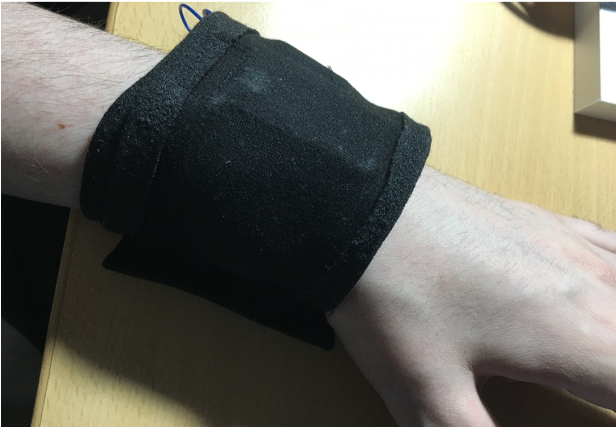
\includegraphics[width=\textwidth]{pics/wristband2.png}
    \caption{Armband angezogen}
    \label{fig:wristband2}
\end{figure}

Damit man Vibrationen {\"u}berhaupt darstellen kann, h{\"a}tte man sich ein eigenes Taktiles Device entwerfen m{\"u}ssen. In meinem Fall war dies nicht n{\"o}tig, da das Wearable vom TECO vorgegeben war. Die Komponenten des Wearables sind zwei Taktoren (TI TLC5971), einen Mikroprozessor (nRF51822 / BLE Nano) und eine Batterie.

Die Kommunikation des Armbands konnte man {\"u}ber eine Serielle Schnittstelle, sowie {\"u}ber Bluetooth Low Energie (LE) realisieren.
Bei der seriellen Schnittstelle ist ein USB-Kabel n{\"o}tig gewesen um den PC mit dem Wearable anzusprechen, dabei w{\"a}re die Mobilit{\"a}t verloren gegangen. Daher habe man die verf{\"u}gbare BLE Schnittstelle benutzt um zwischen dem PC und dem Wearable zu kommunizieren. 

Bluetooth LE {\"u}bertr{\"a}gt Nachrichten nur in einer maximalen Gr{\"o}{\ss}e von 20 Bytes. Diese werden jeweils als zwei Bytes Bl{\"o}cke {\"u}bertragen. 

Anhand der Begrenzung der Daten{\"u}bertragung hat man sich eine geeignete Dekodierung des Signals {\"u}berlegen m{\"u}ssen. 

Die Programmiersprache um die Kommunikation zwischen dem PC und dem Wearable aufzubauen, konnte frei gew{\"a}hlt werden. 
Dabei habe man zuvor verschiedenste Programmiersprachen untersucht. 
Java hat man nach fehlenden Informationen zum Kommunikationsaufbau ausgeschlossen.
%Java hat man nach fehlenden Informationen zum Kommunikationsaufbau ausgeschlossen. 
Schließlich hat man sich f{\"u}r C\# entschieden, da hier ausführliche Dokumentationen vorhanden waren, man erfolgreich eine funktionierende Kommunikation realisiert hat und man gleichzeitig eine Grafische Benutzeroberfl{\"a}che nutzen konnte, die für die spätere Studie hilfreich sein könnte.
%eine funktionierende Kommunikation aufgebaut hat und man gleichzeitig die Grafische Benutzeroberfl{\"a}che nutzen kann um Studie darin durchzuf{\"u}hren. 

Dabei musste herausfinden was f{\"u}r Einstellungsm{\"o}glichkeiten man am Wearable hat. Diese waren die L{\"a}nge und die St{\"a}rke eines Signals.

\paragraph{Signale}

Ein Signal repr{\"a}sentiert eine Vibration, die auf dem Wearable abgespielt wird. Es hat sich die Frage gestellt, wie personalisiert man denn jetzt Signale. Dabei hat man das Signal in drei verschiedene L{\"a}ngen definiert, \textbf{Kurz}, \textbf{Mittel} und \textbf{Lang}. 

Dabei hat man als Vorgabe gehabt, dass man einen Evolution{\"a}ren Algorithmus (EA) benutzen sollte.
Diesen EA hat man verwendet, um f{\"u}r die Signaltypen ein personalisierten Wert zu bestimmen.

Man hat sich ein Vorgang {\"u}berlegen m{\"u}ssen, um f{\"u}r den EA eine Startpopulation zu erzeugen; die Individuen der Population zu bewerten; mittels einer Fitnessfunktion den Fitnesswert f{\"u}r jedes Individuum berechnen; eine geeignete Selektion, Reproduktion und Mutation, sowie die Terminierungsbedingung zu bestimmen. 

Eine geeignete Signalrepr{\"a}sentation musste definiert werden um Signale vom PC zum Wearable {\"u}ber BLE zu senden und abspielen zu lassen. Das bedeutet sowohl am PC als auch am Wearable selbst musste dies definiert werden.

\paragraph{Studie}

Es sollte eine Grafische Oberfl{\"a}che erstellt werden, damit der Proband die Studie komplett {\"u}ber das Programm durchf{\"u}hren kann, indem er die Instruktionen des Programms folgt.

Es hat sich durch das Definieren der Signale und dem EA ergeben, dass die Studie in drei Schritten unterteilt wird. 
In dem ersten Schritt muss man Grenzen f{\"u}r die Erzeugung einer Startpopulation f{\"u}r einen EA bestimmen 
%Der erste Schritt ist es, die Grenzen f{\"u}r eine Startpopulation f{\"u}r einen EA zu bestimmen. 
Der zweite Schritt ist es, einen genetischen Wert f{\"u}r die eigentliche Studie zu bestimmen, dies passiert durch ausf{\"u}hren mehrerer Generationen des EA. 
Schließlich ist der letzte Schritt, dass man sich eine Folge von generische und genetische Signale definiert, die man anschließend vom Benutzer bewerten zu lässt.
%Der letzte Schritt ist es, generische und genetische Signale vom Benutzer bewerten zu lassen.

Alle Daten sollten {\"u}berpr{\"u}ft werden und es sollte herausgefunden werden ob es am signifikante Unterschiede gibt.



%Zu aller erst hat man sich das vorgegebene Armband genauer inspiziert. Dabei konnte man das Armband {\"u}ber eine Serielle Schnittstelle sowie {\"u}ber Bluetooth Low Energie (LE) nutzen. 
%Bei der Nutzung der Seriellen Schnittstelle hatte man zwar den Vorteil, dass man sich nicht mittels Bluetooth auseinander setzen m{\"u}sse, jedoch ist man an einem Kabel {\"u}ber den PC verbunden gewesen, was zur Einschr{\"a}nkung der Bewegungsfreiheit \dots hat. 
%Um genau diesen Nachteil nicht zu haben hat man sich f{\"u}r Bluetooth LE entschieden. 
%Dabei gab es auch einige Nachteile, die man beheben musste. Die Kommunikation mittels Bluetooth LE hatte eine maximale Daten{\"a}bertragung von 20 Bytes. Diese wurden jeweils in zwei Bytes Bl{\"o}cke unterteilt.

%Anhand der Begrenzung der Daten{\"u}bertragung hat man sich eine geeignete Dekodierung des Signals {\"u}berlegen m{\"u}ssen. 











%\dots
%Dabei musste man sich definieren wie ein Signal aufgebaut gewesen ist. Dabei musste f{\"u}r ein Signal eine Datenstruktur erstellt werden. 



%Dekodierung eines Signals.

%Evolution{\"a}rer Algorithmus musste erstellt werden mit allen komponenten, Population Fitness funktion, usw

%Kommunikation mit dem Armband musste aufgebaut werden. 

%Es sollte eine Studie ausgef{\"u}hrt werden um das System zu testen 

%Dabei sollte eine Grafische Oberfl{\"a}che erstellt werden, damit der Benutzer selbst eine Eingabe in den PC machen konnte um n{\"a}chste Signale abspielen zu k{\"o}nnen.

%Es sollten die Daten ausgewertet werden.



%% ==============================
\section{Existierende L{\"o}sungsans{\"a}tze}
%% ==============================
\label{ch:Analyse:sec:RelatedWork}

Hier kommt eine ausf{\"u}hrliche Diskussion
von "`Related Work"'.


%% Existierende L{\"o}sungsans{\"a}tze.tex
%% $Id: Existierende L{\"o}sungsans{\"a}tze.tex 28 2007-01-18 16:31:32Z bless $



%% ==============================
%\section{Weiterer Abschnitt}
%% ==============================
%\label{ch:Analyse:sec:Abschnitt}

%Bla fasel\ldots hat auch schon \cite{TB2000} gesagt und
%\cite{TB98,JSAC96,qosr} sollte man mal gelesen haben.
%Abbildung~\ref{fig:test} auf S.~\pageref{fig:test} sollte man
%sich mal anschauen.

%%% Weiterer Abschnitt.tex
%% $Id: WeitererAbschnitt.tex 28 2007-01-18 16:31:32Z bless $

% System aufbau / ausführung der Studie / analyse aufbau
% beschreibt, was ich gemacht habe.

%Blindtext Blindtext Blindtext Blindtext Blindtext Blindtext Blindtext
%Blindtext Blindtext Blindtext\index{Blindtext} Blindtext Blindtext Blindtext Blindtext

%\begin{figure}[!htbp]
%  \centering
%  \fbox{\parbox{0.8\textwidth}{
%  Abbildungen sollten m{\"o}glichst als EPS (Encapsulated Postscript) 
%  bzw. PDF eingebunden werden.
%  Zur Erzeugung sauberer EPS-Dateien empfiehlt sich das Tool \texttt{ps2eps}
%  zur Nachbearbeitung von Postscript-Dateien. Mit \texttt{epstopdf} kann
%  dann eine PDF-Datei zum Einbinden erzeugt werden.}}
%  \caption{Testabbildung}
%  \label{fig:test}
%\end{figure}

%Blindtext Blindtext Blindtext Blindtext Blindtext Blindtext Blindtext
%% ==============================
\section{Zusammenfassung}
%% ==============================
\label{ch:Analyse:sec:zusammenfassung}

Am Ende sollten ggf. die wichtigsten Ergebnisse nochmal in \emph{einem}
kurzen Absatz zusammengefasst werden.

%% Zusammenfassung.tex
%% $Id: Zusammenfassung.tex 28 2007-01-18 16:31:32Z bless $




%%% Local Variables: 
%%% mode: latex
%%% TeX-master: "diplarb"
%%% End: 


%% entwurf.tex
%% $Id: entwurf.tex 28 2007-01-18 16:31:32Z bless $
%%

\chapter{Entwurf}
\label{ch:Entwurf}
%% ==============================
In diesem Kapitel erfolgt die ausführliche Beschreibung des eigenen
Lösungsansatzes. Dabei sollten Lösungsalternativen diskutiert und
Entwurfsentscheidungen dargelegt werden.


Bla fasel\ldots

%% ==============================
\section{Abschnitt 1}
%% ==============================
\label{ch:Entwurf:sec:Abschnitt1}

Bla fasel\ldots


%% Abschnitt1.tex
%% $Id: Abschnitt1.tex 28 2007-01-18 16:31:32Z bless $
%%

%% ==============================
\section{Ausführung des Programms}
%% ==============================
\label{ch:Entwurf:sec:Ausführung des Programms}

Zu Beginn musste man sich über alles einen Überblick schaffen. 
Das heißt, dass man sich alle Bestandteile einzeln betrachten musste bevor man alles zusammen setzen konnte. 
Es gibt drei / vier große Bestandteile die ich mir überlegen musste.

Zualler erst musste man sich mit dem Armband beschäftigen, um herauzufinden, was es alles konnte. 
Man konnte die Zeit, die das Armband vibrieren sollte festlegen, sowie auch die Stärke, wie Stark das Armband vibrieren sollte. 
Man musst darauf achten, dass man die 20 Bytes, die man lediglich mit Bluethooth übertragen konnte nicht überschreitet.

Als nächstes habe ich mir erst einmal überlegt, wie ich die Daten repräsentieren sollte. Ich habe mir überlegt, dass ich eine Datenstruktur erstellen müsste um das Signal anschließend über BLE an das Armband zu übertragen. Aber wie sehen Signale aus? Zuerst habe ich mir überlegt, was ist die Maximale und Minimale Länge, die ich übertragen werde. Dabei habe ich mich für einen Minimalen Wert von 100 Millisekunden (ms) und eine Maximale Länge von 1024 ms entschieden. Da man das Armabnd auch in verschiedenen Vibrationsstärken abspielen konnte, habe ich herausgefunden, manche Vibrationsstärken gar keine Vibration abspielten, weil so wenig Strom übertragen wurde, dass die Vibrationsmotoren gar nicht erst angesteuert wurden. Dabei haben sich die Grenzen hierbei von 0x07FF bis 0xFFFF behandelt. Um jedoch merkbare unterschiede der Vibrationsstärke zu bestimmen habe ich mir die Grenzen in 5 Bereiche aufgeteilt. 
Somit hatte ich zwei Variablen, die ich für meine Darstellung von einem Signal entscheidend war. 

Da ich jetzt Signale mit einer Länge von 100 ms bis 1024 ms hatte musste ich mir überlegen, wie viele Signaltpyen ich hier erzeugen würde. Der Morsecode beispielsweise bestand aus 3 Teilen ein Kurzes Signal, ein Langes Signal und einer Pause. Dabei wollte ich jetzt nicht den Morsecode nehmen und habe mich für eine eigene Definition entschieden. Dabei habe ich gesagt dass es drei Signaltypen gibt. Diese drei Signaltypen sind Kurz, Mittel und Lang, auf die ich gleich noch einmal zu sprechen komme.

Vorher will ich auf den Evolutionären Algorithmus zu sprechen kommen. Beim Evolutionären Algorithmus musste man sich zu beginn eine Anfangspopulation erstellen. Also in meinem Fall wäre die Anfangspopulation eine Menge von Signalen die eine Variation aufweisen sollte. Wie sollte eine solche Population aussehen? Hier ist mir der Gedanken gekommen, man sollte die Signaltypen in Grenzen aufteilen, das bedeutet, dass man beispielsweise von 100 bis 300 ms Kurz, von 400 bis 700 ms Mittel und von 800 bis 1024 ms Lang definieren sollte. Am Anfang habe ich dies auch gemacht, dass die Grenzen fest von mir vorgegeben waren, jedoch  hat man festgestellt, dass die Nutzer nicht genau diese Grenzen als Kurz, Mittel und Lang empfunden haben. Das heißt man musste sich vor dem Evolutionören Algorithmus überlegen, wie die Nutzer die Signalgrenzen selbst bestimmten. (Nähere Information im Kapitel Implementierung)

Nach der Bestimmung der Signaltypen, hat man sich erneut an den Evolutionären Algorithmus gewagt. Das bedeutete, man musste eine Anfangspopulation bestimmen. Dabei hat man N Individuen für jeden Signaltypen innerhalb seiner Grenzen erzeugt. Zuerst komplett zufällig innerhalb der Grenzen, dabei kam man zu dem Ergebnis, dass die Grenzen nur in seltenen fällen drinnen waren. D.h. dass man nie den vollständigen Intervall den man vorher bestimmt hat in der Anfangspopulation vertreten war. Deshalb habe man von den N Individuen zwei Individuen erzeugt, die genau die beiden Grenzen repräsentiert haben.

Nach der Erzeugung der Anfangspopulation sollten die Signale vom Benutzer alle bewertet werden. 
Dabei hatte man den Gedanken, dass man den Benutzer die Signale mehrmals abspielt und ihn jedes mal abfragt, was für ein Signal er erkannt hat und anhand der Häufigkeit, die er das Signal als den Signaltypen erkannt hat wie das Programm es für Ihn im Vorfeld bestimmt hatte, einen Fittnesswert bestimme. Jedoch müssten diese 3*N Signale mehrmals abgespielt werden, um eine Häufigkeit zu erhalten. Wenn man hier für die Population jedes Individuum fünf mal abspielen würde, wäre man bei 15*N. Bei einem N von 10 Signalen pro Signaltyp wären dass dann 150 Bewertungen die der Nutzer pro Population machen müsste um nur eine Generation zu bewerten. Wenn man nur vier Generationen bestimmen wollte, so wäre man bei 450 Bewertungen nur um einen personalisierten Wert zu erhalten. Das wäre für einen normalen Benutzer nicht zumutbar, dass er so viel Zeit in anspruch nehmen würde um so viele Signale zu bewerten. 

Daher musste eine alternative her. Die Alternative ist gewesen, man spiele dem Benutzer jedes Individuum nur einmal ab und stellt Ihn dazu drei Fragen, die wie in einem SUS Fragebogen gestellt wird, mit einer Skala von sehr gut bis sehr schlecht. [BILD EINFÜGEN]
Anhand der Fragen habe ich einen Fitnesswert bestimmt. Die weitere Beschreibung des Algorithmus wird in der Implementierung beschrieben.

Mit jeder Generation ist man davon ausgegangen, dass die Grenzen der Signaltypen kleiner wurde und zu dem Wert, dass dem Nutzer am besten gefallen würde hinkonvergieren würde.
 Würde man dies weitertreiben, bis die jeweiligen Signaltypen gegen eine Zahl konvergieren, würde man noch ein paar mehr Itterationen machen müssen, was unter Bedacht, dass der Benutzer nicht so lange die Signale bewerten würde nach vier Itterationen aufgehort. Nachdem der Algorithmus also nach der vierten Generation die Population erzeugt hat, wurde von allen Individuen das Minumin und Maximum der jeweiligen Signaltypen bestimmt worden. Anhand der Minima und Maxima wurde für jeden Signaltypen der Mittelwert bestimmt.

Somit hat man nach dem Algorithmus einen personalisierten Kurz, Mittel und Lang Wert.

Im dritten Schritt musste man herausfinden, wie die Signale im Vergleich zu Vorgegebenen Werten erkannt werden.
Dabei hat man verschiedene Folgen von Signalen vordefiniert, die der Benutzer erkennen sollte. Dabei habe man zuerst drei Signal-Folgen (aka Muster) abgespielt, anschließend vierer Muster und zu letzt fünfer Muster. Es wurde abwechselnd ein zufälliges genetisches Muster und ein generisches Muster abgespielt. 

%% ==============================
\section{Abschnitt 2}
%% ==============================
\label{ch:Entwurf:sec:Abschnitt2}

Bla fasel\ldots


Blindtext Blindtext Blindtext Blindtext Blindtext Blindtext Blindtext
Blindtext Blindtext Blindtext Blindtext Blindtext Blindtext Blindtext
Blindtext Blindtext Blindtext Blindtext Blindtext Blindtext Blindtext
Blindtext Blindtext Blindtext Blindtext Blindtext Blindtext Blindtext
Blindtext Blindtext Blindtext Blindtext Blindtext Blindtext Blindtext
Blindtext Blindtext Blindtext Blindtext Blindtext Blindtext Blindtext
Blindtext Blindtext Blindtext Blindtext Blindtext Blindtext Blindtext
Blindtext Blindtext Blindtext Blindtext Blindtext Blindtext Blindtext
Blindtext Blindtext Blindtext Blindtext Blindtext Blindtext Blindtext
Blindtext Blindtext Blindtext Blindtext Blindtext Blindtext Blindtext
Blindtext Blindtext Blindtext Blindtext Blindtext Blindtext Blindtext
Blindtext Blindtext Blindtext Blindtext Blindtext Blindtext Blindtext
Blindtext Blindtext Blindtext Blindtext Blindtext Blindtext Blindtext
Blindtext Blindtext Blindtext Blindtext Blindtext Blindtext Blindtext
Blindtext Blindtext Blindtext Blindtext Blindtext Blindtext Blindtext
Blindtext Blindtext Blindtext Blindtext Blindtext Blindtext Blindtext
Blindtext Blindtext Blindtext Blindtext Blindtext Blindtext Blindtext

Blindtext Blindtext Blindtext Blindtext Blindtext Blindtext Blindtext
Blindtext Blindtext Blindtext Blindtext Blindtext Blindtext Blindtext
Blindtext Blindtext Blindtext Blindtext Blindtext Blindtext Blindtext
Blindtext Blindtext Blindtext Blindtext Blindtext Blindtext Blindtext
Blindtext Blindtext Blindtext Blindtext Blindtext Blindtext Blindtext
Blindtext Blindtext Blindtext Blindtext Blindtext Blindtext Blindtext
Blindtext Blindtext Blindtext Blindtext Blindtext Blindtext Blindtext
Blindtext Blindtext Blindtext Blindtext Blindtext Blindtext Blindtext
Blindtext Blindtext Blindtext Blindtext Blindtext Blindtext Blindtext
Blindtext Blindtext Blindtext Blindtext Blindtext Blindtext Blindtext
Blindtext Blindtext Blindtext Blindtext Blindtext Blindtext Blindtext
Blindtext Blindtext Blindtext Blindtext Blindtext Blindtext Blindtext
Blindtext Blindtext Blindtext Blindtext Blindtext Blindtext Blindtext
Blindtext Blindtext Blindtext Blindtext Blindtext Blindtext Blindtext
Blindtext Blindtext Blindtext Blindtext Blindtext Blindtext Blindtext
Blindtext Blindtext Blindtext Blindtext Blindtext Blindtext Blindtext
Blindtext Blindtext Blindtext Blindtext Blindtext Blindtext Blindtext
Blindtext Blindtext Blindtext Blindtext Blindtext Blindtext Blindtext
Blindtext Blindtext Blindtext Blindtext Blindtext Blindtext Blindtext
Blindtext Blindtext Blindtext Blindtext Blindtext Blindtext Blindtext

Blindtext Blindtext Blindtext Blindtext Blindtext Blindtext Blindtext
Blindtext Blindtext Blindtext Blindtext Blindtext Blindtext Blindtext
Blindtext Blindtext Blindtext Blindtext Blindtext Blindtext Blindtext
Blindtext Blindtext Blindtext Blindtext Blindtext Blindtext Blindtext
Blindtext Blindtext Blindtext Blindtext Blindtext Blindtext Blindtext
Blindtext Blindtext Blindtext Blindtext Blindtext Blindtext Blindtext
Blindtext Blindtext Blindtext Blindtext Blindtext Blindtext Blindtext
Blindtext Blindtext Blindtext Blindtext Blindtext Blindtext Blindtext
Blindtext Blindtext Blindtext Blindtext Blindtext Blindtext Blindtext
Blindtext Blindtext Blindtext Blindtext Blindtext Blindtext Blindtext
Blindtext Blindtext Blindtext Blindtext Blindtext Blindtext Blindtext
Blindtext Blindtext Blindtext Blindtext Blindtext Blindtext Blindtext
Blindtext Blindtext Blindtext Blindtext Blindtext Blindtext Blindtext
Blindtext Blindtext Blindtext Blindtext Blindtext Blindtext Blindtext
Blindtext Blindtext Blindtext Blindtext Blindtext Blindtext Blindtext

Blindtext Blindtext Blindtext Blindtext Blindtext Blindtext Blindtext
Blindtext Blindtext Blindtext Blindtext Blindtext Blindtext Blindtext
Blindtext Blindtext Blindtext Blindtext Blindtext Blindtext Blindtext
Blindtext Blindtext Blindtext Blindtext Blindtext Blindtext Blindtext
Blindtext Blindtext Blindtext Blindtext Blindtext Blindtext Blindtext
Blindtext Blindtext Blindtext Blindtext Blindtext Blindtext Blindtext
Blindtext Blindtext Blindtext Blindtext Blindtext Blindtext Blindtext
Blindtext Blindtext Blindtext Blindtext Blindtext Blindtext Blindtext
Blindtext Blindtext Blindtext Blindtext Blindtext Blindtext Blindtext
Blindtext Blindtext Blindtext Blindtext Blindtext Blindtext Blindtext
Blindtext Blindtext Blindtext Blindtext Blindtext Blindtext Blindtext
Blindtext Blindtext Blindtext Blindtext Blindtext Blindtext Blindtext
Blindtext Blindtext Blindtext Blindtext Blindtext Blindtext Blindtext
Blindtext Blindtext Blindtext Blindtext Blindtext Blindtext Blindtext
Blindtext Blindtext Blindtext Blindtext Blindtext Blindtext Blindtext
Blindtext Blindtext Blindtext Blindtext Blindtext Blindtext Blindtext

Blindtext Blindtext Blindtext Blindtext Blindtext Blindtext Blindtext
Blindtext Blindtext Blindtext Blindtext Blindtext Blindtext Blindtext
Blindtext Blindtext Blindtext Blindtext Blindtext Blindtext Blindtext
Blindtext Blindtext Blindtext Blindtext Blindtext Blindtext Blindtext
Blindtext Blindtext Blindtext Blindtext Blindtext Blindtext Blindtext
Blindtext Blindtext Blindtext Blindtext Blindtext Blindtext Blindtext
Blindtext Blindtext Blindtext Blindtext Blindtext Blindtext Blindtext
Blindtext Blindtext Blindtext Blindtext Blindtext Blindtext Blindtext
Blindtext Blindtext Blindtext Blindtext Blindtext Blindtext Blindtext
Blindtext Blindtext Blindtext Blindtext Blindtext Blindtext Blindtext
Blindtext Blindtext Blindtext Blindtext Blindtext Blindtext Blindtext
Blindtext Blindtext Blindtext Blindtext Blindtext Blindtext Blindtext
Blindtext Blindtext Blindtext Blindtext Blindtext Blindtext Blindtext

%% ==============================
\section{Zusammenfassung}
%% ==============================
\label{ch:Entwurf:sec:zusammenfassung}

Am Ende sollten ggf. die wichtigsten Ergebnisse nochmal in \emph{einem}
kurzen Absatz zusammengefasst werden.

%%% Local Variables: 
%%% mode: latex
%%% TeX-master: "diplarb"
%%% End: 


%% implemen.tex
%% $Id: implemen.tex 4 2005-10-10 20:51:21Z bless $
%%

\chapter{Implementierung}
\label{ch:Implementierung}
%% ==============================

%% ==============================
%\section{Signal}
%% ==============================
\label{ch:Implementierung:sec:Signal}


%% Signale.tex
%% $Id: Signale.tex 4 2005-10-10 20:51:21Z bless $
%%

Das Kapitel \textbf{Implementierung} wird anhand dem im Entwurf besprochenen Verlauf der Studie erkl{\"a}rt.

Bei der Entwicklung des Programms hat man sich Gedanken {\"u}ber ein System gemacht, bei dem man die Ganzen Daten schon digital abgespeichert hat und nicht noch Informationen vom Probanden vom Zettel per Hand in den PC eintragen muss. Aus diesem Grund hat man sich f{\"u}r eine Grafische Benutzeroberfl{\"a}che, auch kurz GUI (graphical user interface) genannt, entschieden. 
Die Programmiersprache die verwendet wurde ist C\# gewesen.
Der Entstehungsprozess wurde auf Papier entworfen. Das Design sollte schlicht und einfach sein und den Fokus auf das Programm und nicht auf andere Komponenten des Betriebsystems ablenken. Die Papier Skizzen sind im Anhang vorhanden.

\paragraph{Informationen zur Person}
Bei den Nachforschungen des Studiendesigns \cite{benyon2005designing}, habe man sich nach mehreren Entw{\"u}rfen f{\"u}r folgende Fragen entschieden:

\begin{itemize}
\item Wie alt sind Sie?
\item Angabe des Geschlechts
\item Empfinden Sie sich als musikalisch? 
\item Spielen Sie gelegentlich Computer Spiele?
\item Haben Sie Erfahrungen mit Taktilen Ger{\"a}ten?
\item Haben Sie schon einmal eine Smartwatch verwendet?
\end{itemize}

Da man f{\"u}r den Probanden nicht mit allen Fragen auf einmal {\"u}berh{\"a}ufen wollte, hat man diese Fragen auf zwei Seiten dargestellt \autoref{AngabenZurPerson}. Im Hintergrund hatte man eine einfache Klasse \textbf{Person}, die die Informationen der Antworten dieser Befragung gespeichert hat. Um zu vermeiden, dass Daten verloren gehen, habe man die Daten zur Person schon nach diesem Schritt in einer externen Datei gespeichert. F{\"u}r jeden Probanden hat man im Vorfeld eine anonyme Datei angelegt, die im Nachhinein nicht auf den Probanden zur{\"u}ckschlie{\ss}en zu k{\"o}nnen.  

\begin{figure}[htbp] 
	\centering
	\begin{minipage}[t]{0.45\textwidth}
		\includegraphics[width=\textwidth]{pics/gui/{AngabenZurPerson1}.png}
	\end{minipage}
	\begin{minipage}[t]{0.45\textwidth}
		\includegraphics[width=\textwidth]{pics/gui/{AngabenZurPerson2}.png}
	\end{minipage}
	\caption{GUI f{\"u}r die Befragung zu den Angaben zur Person}
	\label{fig:AngabenZurPerson}
\end{figure}

\paragraph{Signal}
Wie schon im Entwurf beschrieben, ist das Signal eines der wichtigsten Bestandteile des Programms.
%Das Signal ist wie im Entwurf schon beschrieben, einer der wichtigsten Bestandteile meines Programms. 

Ein \textbf{Signal} besitzt die Attribute L{\"a}nge in ms, St{\"a}rke, die den jeweiligen Zustand der St{\"a}rke speichert \autoref{zdiagramm}, den Signaltypen, sowie die Grenzen des Signaltypens und die Anzahl wie oft ein Signal erneut abgespielt wurde. 
Da man in den n{\"a}chsten beiden Phasen dem Signal einen Signaltypen zuordnen soll, wurde daf{\"u}r auch ein weiteres Attribut angelegt, sowie die Zeit, die ben{\"o}tigt wurde um die Frage zu beantworten.
%Jedes Signal beinhaltet die Attribute L{\"a}nge, St{\"a}rke, der Signaltyp sowie die Grenzen des Signaltyps.

In der Phase indem der Algorithmus durchgef{\"u}hrt wird, werden noch zwei zus{\"a}tzliche Fragen gestellt f{\"u}r die man in der Klasse \textbf{Signal} auch noch diese beiden Werte gespeichert hat.

%Je nach dem in welcher Phase des Programms man sich gerade befindet, werden noch weitere Attribute gespeichert
%Das Programm besteht aus vier Phasen.

\paragraph {Bestimmung der Grenzen durch Bewertung durch den Nutzer}

Nachdem der Proband die Angaben zur Person beantwortet hat, erscheint ein Benachrichtigungsfenster, indem Informationen {\"u}ber den die aktuelle Phase erkl{\"a}rt sind. 
Falls der Proband zu einem Zeipunkt Fragen haben sollte, werden diese durch den Aufseher beantwortet.
F{\"u}r die Bestimmung der Grenzen wurden 10 Signale erzeugt, die gleichverteilt sind. 
Mithilfe einer Zufallsfunktion werden diese Signale zuf{\"a}llig ausgew{\"a}hlt und in dieser Reihefolge abgespielt. 
Der Proband soll f{\"u}r jeden der 10 Signalen einen der Signaltypen \textbf{Kurz}, \textbf{Mittel} oder \textbf{Lang} zuordnen. 
Dabei habe man die im Entwurf besprochenen Sonderf{\"a}lle {\"u}berpr{\"u}ft und bei erfolgreicher Bildung der Grenzen ist man in die n{\"a}chste Phase {\"u}bergegangen.
%Als alle 10 Signale bewertet wurden, hat man {\"u}berpr{\"u}ft, ob der Kleinste Wert von 100ms Kurz und der gr{\"o}{\ss}te Wert von 1000ms Lang gewesen ist. 

Wenn die Bestimmung der Grenzen nicht erolgreich gewesen ist, wird der Benutzer gebeten die gleiche zuf{\"a}llige Reihenfolge erneut zu bewerten. 

Sollte ein Proband den Replay-Button dr{\"u}cken, wird das letzte Signal erneut abgespielt.

F{\"u}r die GUI \autoref{GrenzenBestimmen} hat man sich auf das wesentliche beschr{\"a}nkt. Die Anweisung an den Benutzer, hat immer den gleichen Text dargestellt. Als Antwortm{\"o}glichkeiten des Signals wurden je ein Radio-Button erstellt, der einen der Signaltypen repr{\"a}sentierte. Ist in jeder Phase, inder ein Signal abgespielt wurde, wurde der Replay-Button immer an der gleichen Position plaziert. 

Der Ablauf einer Bewertung ist wie folgt abgelaufen, nach der Best{\"a}tigung des Benachrichtigungsfenster wurden im Hintergrund die Signale in zuf{\"a}lliger Reihenfolge erstellt. Darauf wurde das erste Signal {\"u}ber BLE an das Wearable gesendet. Das Wearable hat dieses Signal empfangen, ausgewertet und hat die Informationen als Vibration abgespielt. Das was der Benutzer dadurch empfunden hat wurde {\"u}ber den PC mittels der Maus bewertet. Nach einer Bewertung gab es keine M{\"o}glichkeit die Bewertung eines vorherigen Signals erneut anzupassen. Nachdem das Signal vom Probanden bewertet wurde, wurde der Maus-Cursor durch dem Programm an eine Anfangsposition gesetzt, damit der Benutzer doppelt auf ein Radio-Button dr{\"u}cken konnte. Um dem Probanden zu signalisieren, dass er die Checkbox gedr{\"u}ckt hat, hat man die Check-Box einen Augenblick visuell markiert gelassen, nachdem man den Maus-Cursor neu positioniert hat. Mit der Neupositionierung der Maus hat man erreicht, dass man immer den gleichen Weg hatte um die Checkboxen zu erreichen, aber man hatte auch nach mehreren Fragen die Maus anheben weiter nach oben legen m{\"u}ssen, denn man hat schon das Ende der Tischkannte erreicht.

\begin{figure}
	\centering
    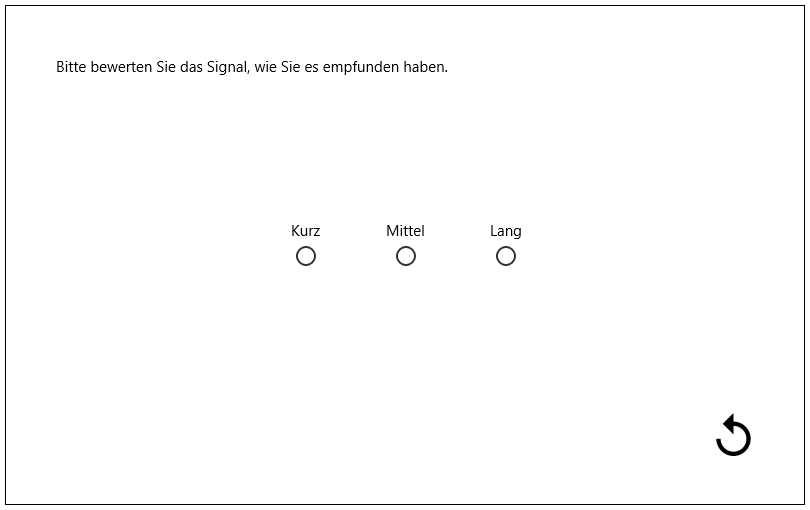
\includegraphics[width=\textwidth]{pics/gui/GrenzenBestimmen.png}
    \caption{GUI zur Bestimmung der Grenzen}
    \label{fig:GrenzenBestimmen}
\end{figure}

\paragraph {3. Ausf{\"u}hren des Algorithmus}


\begin{figure}[htbp] 
	\centering
	\begin{minipage}[t]{0.45\textwidth}
		\includegraphics[width=\textwidth]{pics/gui/{Algorithmus1}.png}
	\end{minipage}
	\begin{minipage}[t]{0.45\textwidth}
		\includegraphics[width=\textwidth]{pics/gui/{Algorithmus2Emotion}.png}
	\end{minipage}
	\caption{}
	\label{fig:Bild10}
\end{figure}




%\paragraph {1. Aufnahme der Personalien}
%Der erste Schritt bestand darin, den Probanden den Personalien zu fragen. 

%\paragraph {2. Bestimmung der Grenzen durch Bewertung durch den Nutzer}
%\paragraph {3. Ausf{\"u}hren des Algorithmus}
\paragraph {4. Muster Erkennung} 

%Das Signal ist ein wichtiger Bestandteil meines Programm. 
Ein Signal beinhaltet die Signall{\"a}nge, die in Millisekunden gespeichert wird, und eine Signalst{\"a}rke, die in 5 St{\"a}rkestufen eingeteilt ist. 



Ich habe meinen Evolution{\"a}ren Algorithmus so angepasst, dass bei mir ein Induviduum ein Signal ist. 
Ich habe dem Benutzer das Signal mit dem Wearable abspielen lassen und im Anschluss Fragen beantworten lassen. 
Er sollte bewerten wie gut er das Signal erkannt hat. Die Bewertung vom Benutzer war entscheidend um nach der kompletten Bewertung der Population 

% -----------------------------------------------------------------------

%\paragraph {1. Aufnahme der Personalien}


%Um in der Evaluierung m{\"o}gliche Erkentnisse zwischen bestimmten Benutzergruppen herausfinden zu k{\"o}nnen, hat man dem Benutzer Eine Reihe von Fragen gestellt, die im Bild XXXX zu sehen sind.
%Diese Daten wurden anonymisiert gespeichert. 

%\paragraph {2. Bestimmung der Grenzen durch Bewertung durch den Nutzer}


%\paragraph {3. Ausf{\"u}hren des Algorithmus}


%\paragraph {4. Muster Erkennung} 

%MUSTER BILD



%% ==============================
%\section{Muster}
%% ==============================
%\label{ch:Implementierung:sec:Muster}


%%% Signale.tex
%% $Id: Signale.tex 4 2005-10-10 20:51:21Z bless $
%%



%%% Local Variables: 
%%% mode: latex
%%% TeX-master: "diplarb"
%%% End: 


%% eval.tex
%% $Id: eval.tex 5 2005-10-10 20:55:48Z bless $

\chapter{Evaluierung}
\label{ch:Evaluierung}
%% ==============================
%Hier kommt der Nachweis, dass das in Kapitel~\ref{ch:Entwurf}
%entworfene Konzept auch funktioniert. Leistungsmessungen einer
%Implementierung werden auch immer gerne gesehen.


%% ==============================
\section{Studiendesign}
%% ==============================
\label{ch:Implementierung:sec:Studiendesign}

%% Studiendesign.tex
%% $Id: Studiendesign.tex 4 2005-10-10 20:51:21Z bless $
%%

%\chapter{Studiendesign}
%\label{ch:Studiendesign}

%% ==============================
\subsection{Studiendesign}
%% ==============================

\begin{figure}
	\centering
    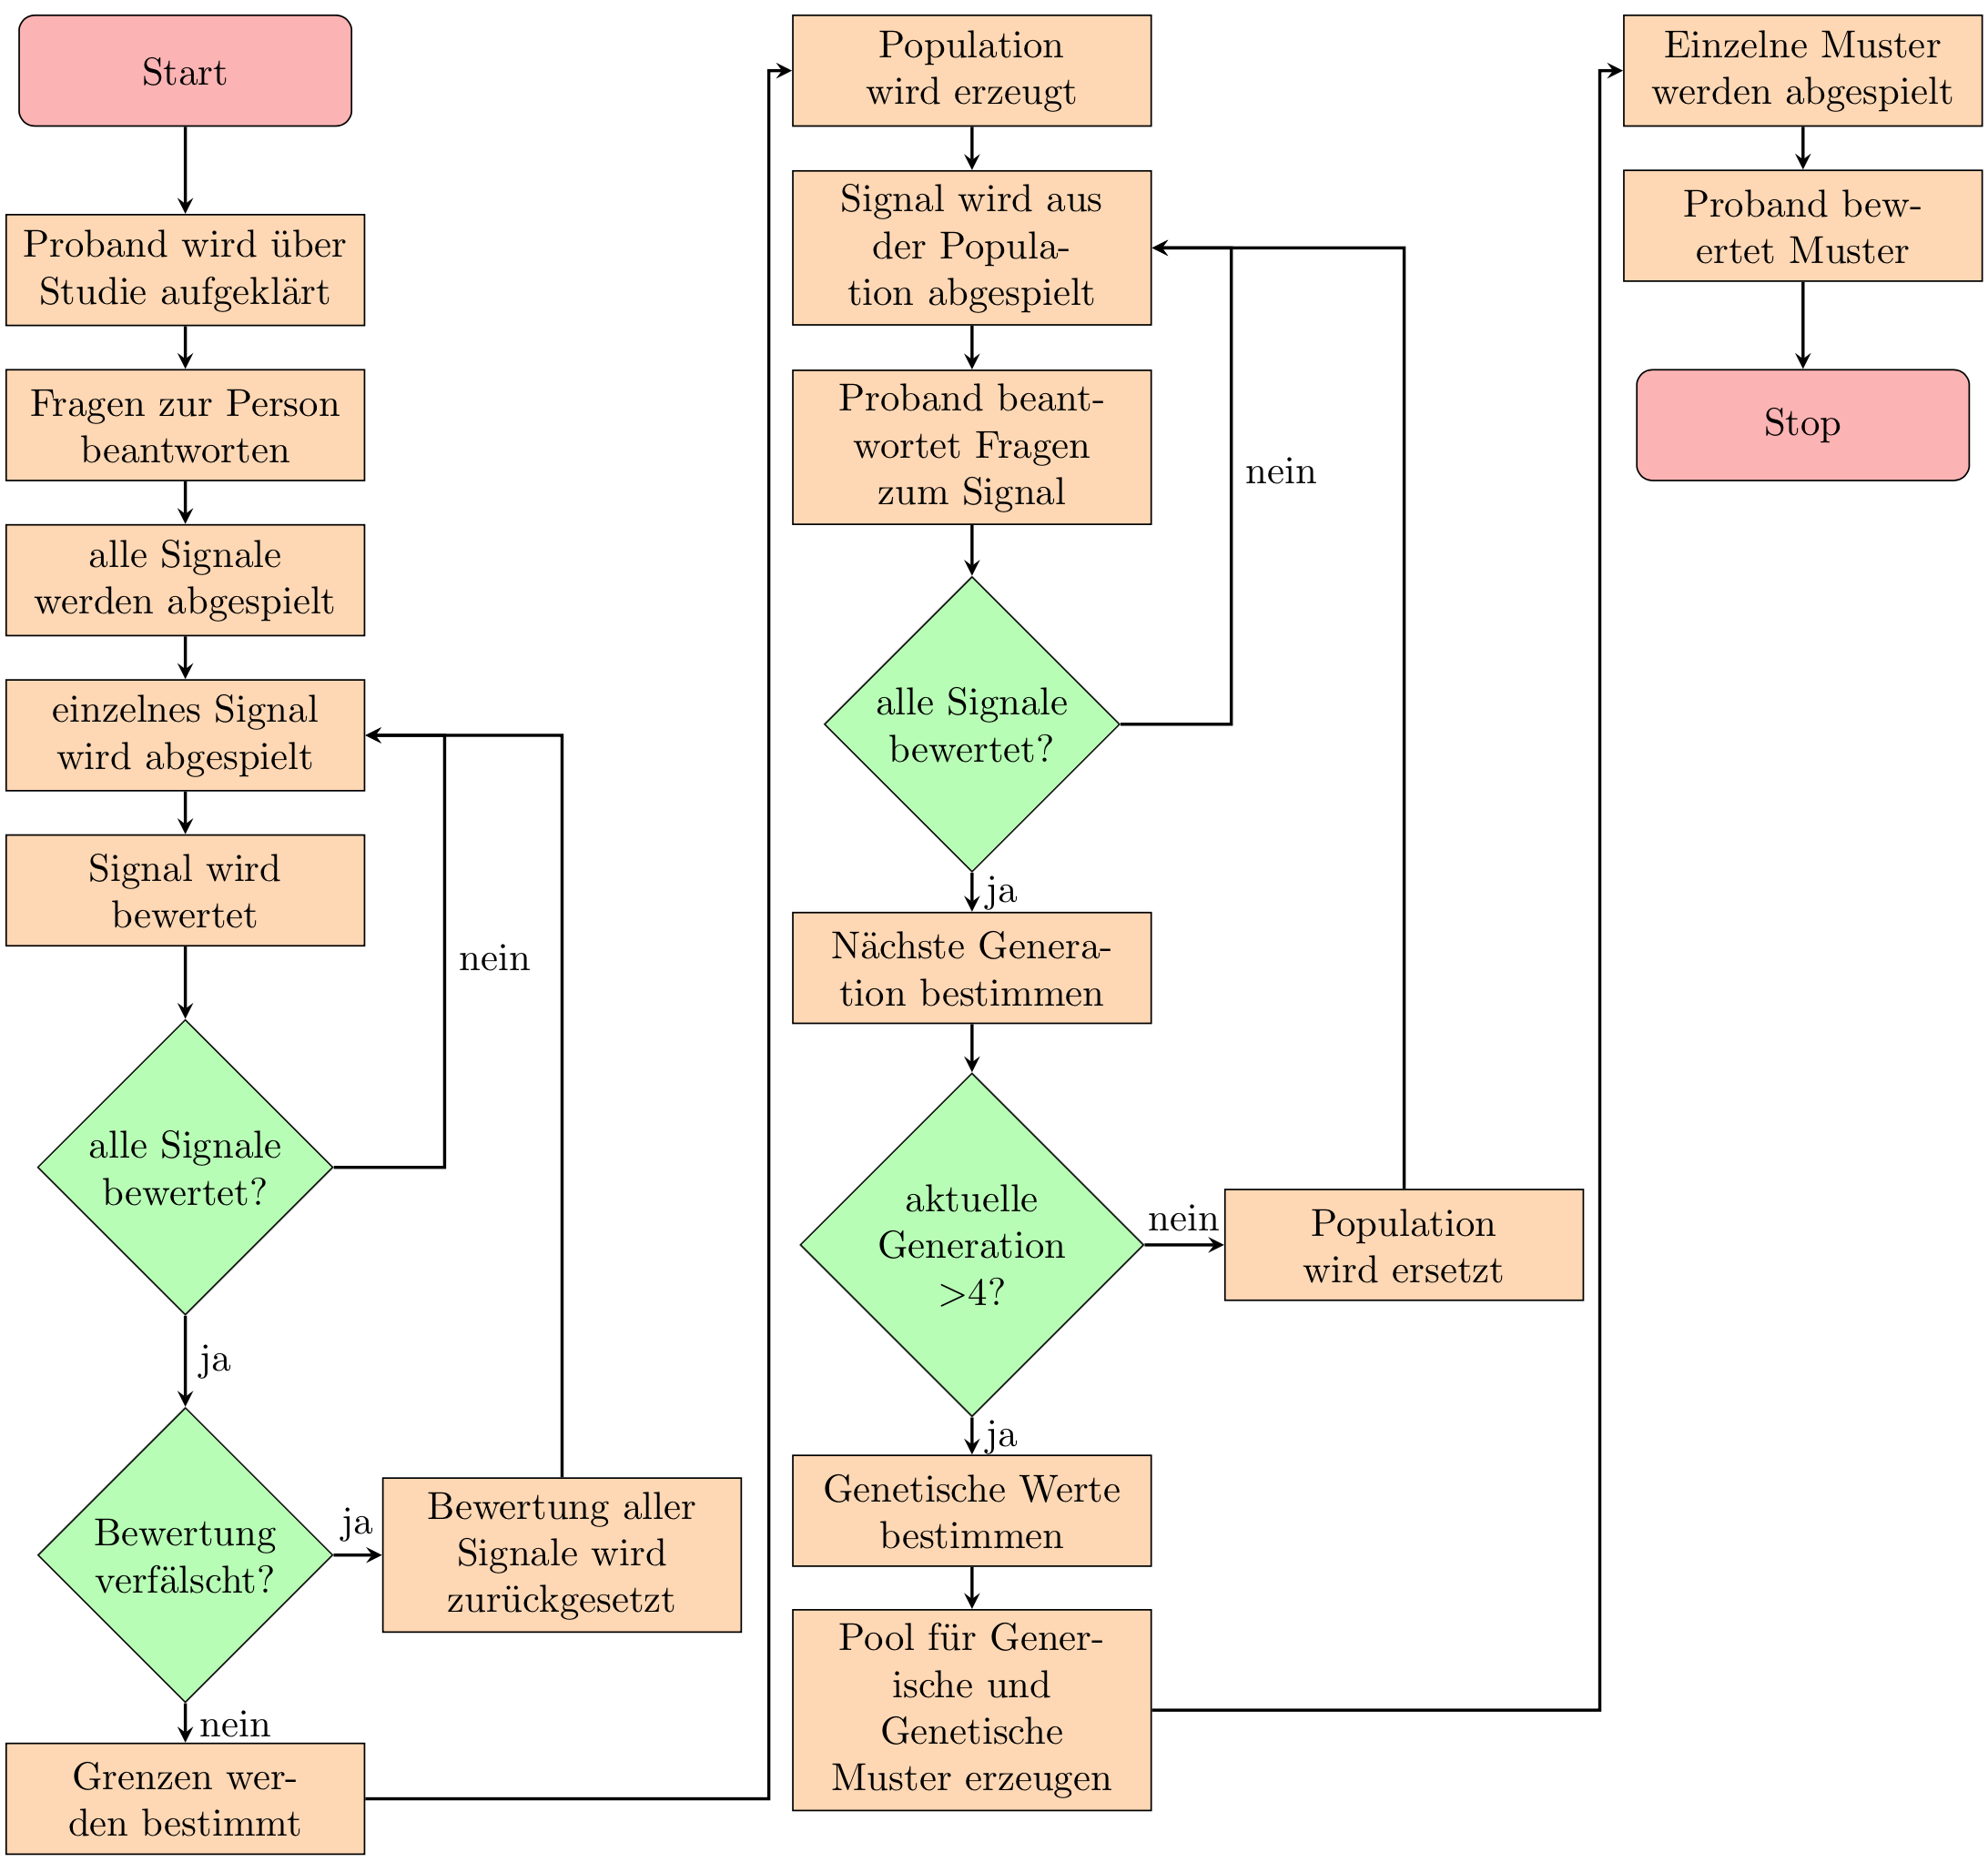
\includegraphics[width=\textwidth]{pics/analyse/Programmablaufdiagramm.png}
    \caption{Studienablauf}
    \label{fig:flussdiagramm}
\end{figure}

Im folgenden Programmablauf \autoref{fig:flussdiagramm} hat man sich orientiert um die Studie zu entwerfen. 
{\"U}ber Mailinglisten und Bekanntenkreis haben sich 32 Probanden bereiterkl{\"a}rt an der Studie teilzunehmen. 
Dabei waren 72 Prozent M{\"a}nner und 28 Prozent Frauen. 
Das Alter der Probanden war zwischen 12 bis 54 Jahren vertreten und das Durchschnittsalter war 22 Jahre \autoref{fig:AngabenZurPerson}.  
Die Studie hat zwischen 30 Minuten und einer Stunde gedauert.
Die Studien wurden an drei verschiedenen Orten durchgef{\"u}hrt, im TECO in Karlsruhe, in einem Seminarraum an der Hochschule Darmstadt und in einem Arbeitszimmer in Meschede.

F{\"u}r jeden teilgenommenen Probanden ist der gleiche Ablauf durchgef{\"u}hrt. 
Vor der Studie wurde ein Termin mit dem Probanden vereinbart. 
Nachdem der Proband zur abgemachten Zeit am vorgegebenen Ort angekommen ist, wurde Ihm erkl{\"a}rt wof{\"u}r die Studie ist, was man mit der Studie herausfinden will und welche Erwartungen man an den Probanden hat. 
Als der Proband alles verstanden hat und die Einverst{\"a}ndniserkl{\"a}rung verstanden und unterschrieben hatte, wurde Ihm das Armband angezogen. Dabei haben die Rechtsh{\"a}nder das Armband an dem linken Arm und die Linksh{\"a}nder an dem rechten Arm angelegt bekommen.

Da man f{\"u}r die Studie ein System mit einer Grafischen Oberfl{\"a}che (GUI) entworfen hatte, wurde der Proband mithilfe des Systems durch die Studie gef{\"u}hrt.
Dabei wurden dem Probanden ein paar Personalien abgefragt, wie das Alter, das Geschlecht, ob sich die Person als Musikalisch empfindet, ob man Computerspiele spielen w{\"a}rde, ob man schon einmal eine Smartwatch benutzt habe und ob die Person schon mal ein Tactiles Ger{\"a}t benutzt habe. 
Falls vom Probanden Fragen w{\"a}hrend der Studie Fragen aufgekommen sind wurden diese sofort beantwortet. 

Nach der Aufnahme der Personalien, wurde dem Benutzer erkl{\"a}rt, was Ihn als n{\"a}chstes erwartet und von Ihm verlangt wird. 
Man hat dem Nutzer im ersten Schritt 10 Signale abgespielt, um Ihn ein Gef{\"u}hl f{\"u}r Signale zu geben. 
Im Anschluss wurde dem Probanden jedes Signal einzeln erneut abgespielt. 
Dabei sollte er das Signal zu drei jeweiligen Kategorien zuordnen, die Kategorien waren die Signaltypen \textit{Kurz}, \textit{Mittel} und \textit{Lang}. 
Dieser Schritt war daf{\"u}r notwendig um f{\"u}r den Benutzer die Grenzen f{\"u}r die jeweilige Kategorien zu bestimmen. 
Diese Grenzen sind f{\"u}r die Initialisierung des Algorithmus notwendig gewesen. 

Als die 10 Signale bewertet wurden, wurde der Benutzer dar{\"u}ber aufgekl{\"a}rt, was Ihm als n{\"a}chsten Schritt erwartet. 
Es wurde Ihm ein anhand seiner vorherigen Eingaben eine Population von Signalen erzeugt, es wurde ein zuf{\"a}lliges Signal abgespielt, dass er bewerten sollte.
Anhand der drei Fragen wurde das Signal bewertet. 
Um eine Itteration komplett zu bewerten wurde dieser Vorgang 30 mal wiederholt. 
Im Anschluss wurde gefragt wie der Benutzer sich derzeit f{\"u}hlt. 
Anhand einer komplett bewerteten Itteration wurde dem Benutzer neue Werte berechnet. 
Es wurden insgesamt vier Itterationen durchgef{\"u}hrt um einen m{\"o}glichst genauen Wert f{\"u}r den Benutzer zu bestimmen.

Im letzten Schritt wurde dem Benutzer aufgekl{\"a}rt, dass ab dem Zeitpunkt nur noch Folgen von Signalen, die man ab jetzt Muster nennt, abgespielt werden.
Die Probanden sollten angeben in welcher Reihenfolge was f{\"u}r Signaltypen abgespielt wurden. 
Es wurde f{\"u}r alle Probanden im Vorfeld alle Muster definiert, damit jeder die gleichen Muster abgespielt bekommt. 
Es gab zwei Arten von Muster, die generischen Muster und die genetischen Muster. 
Der einzige Unterschied zwischen den beiden Arten waren die Werte, die die Signale in einem Muster zugewiesen wurden. 
Das bedeutet es wurden zwei mal das selbe Muster abgespielt mit lediglich anderen Werten. 
Die Genetischen Muster hatten die Werte, die nach dem Algorithmus erzeugt wurden {\"u}bernommen, wobei die generischen Muster einen vordefinierten Wert zugewiesen bekommen hat. 
Der generische Wert ist f{\"u}r jeden Probanden gleich gewesen und hat man sich wie im Entwurf schon beschrieben am Paper \cite{pescara2016ruttelflug} orientiert.
Dabei gab es Muster mit drei, vier und f{\"u}nf Signalen. 
Nacheinander wurde dem Nutzer zuerst alle Muster mit drei Signalen, gefolgt von allen Mustern mit vier und zuletzt alle Muster mit fünf Signalen abgespielt. 
Dabei wurde das genetische Muster abwechselnd zum generischen Muster abgespielt. 

Nachdem alle Muster von dem Probanden bewertet wurden, haben Sie Ihre e-Mail noch auf Papier angegeben um an einer automatischen Verlosung von zwei Gutscheinen teilzunehmen. 
Bei Interesse wurde Ihnen Ihre Werte gezeigt und erkl{\"a}rt, was genau im Hintergrund passiert worden ist. 
W{\"a}hrend der ganzen Studie standen dem Probanden ausreichend S{\"u}{\ss}igkeiten zur Verf{\"u}gung, bei denen Sie sich frei bedienen konnten.




%% ==============================
\section{Analyse}
%% ==============================
\label{ch:Evaluierung:sec:Abschnitt1}
%% 062Analyse.tex
%% $Id: 062Analyse.tex 4 2005-10-10 20:51:21Z bless $
%%

%% ==============================
\subsection{Angaben der Probanden}
%% ==============================

\begin{figure}[htbp] 
	\centering
	\begin{minipage}[t]{0.4\textwidth}
		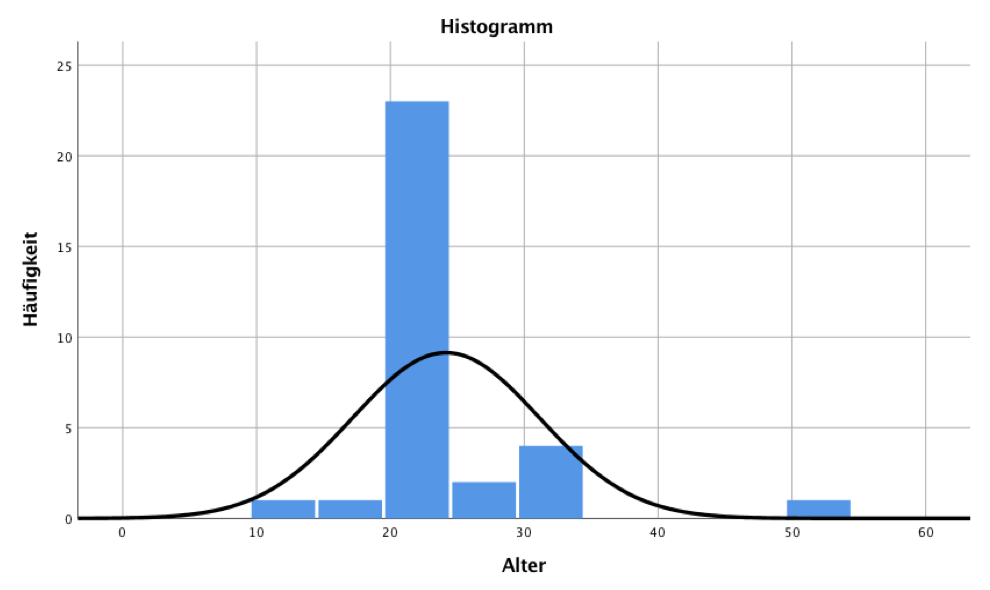
\includegraphics[width=\textwidth]{pics/analyse/person/alter.png}
	\end{minipage}
	\begin{minipage}[t]{0.4\textwidth}
		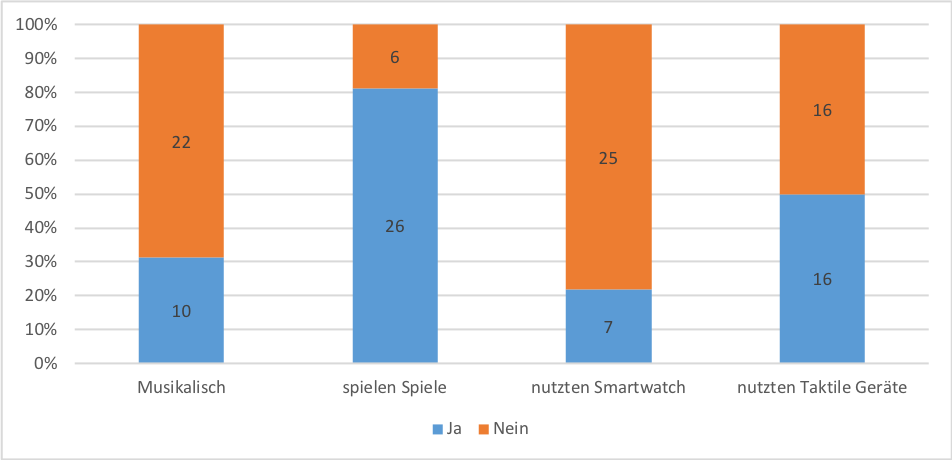
\includegraphics[width=\textwidth]{pics/analyse/person/questions.png}
	\end{minipage}
	\caption{Alter aller Probanden (links) und Auswertung der Fragen (rechts)}
	\label{fig:AngabenZurPerson}
\end{figure}

Nach der Befragung der Probanden hat sich ergeben \autoref{fig:AngabenZurPerson}, dass 31\% musikalisch sind, 81\% gelegentlich Computerspiele spielen. 21\% haben schon mal eine Smartwatch benutzt und genau die h{\"a}lfte haben schon mal taktile Ger{\"a}te benutzt.

%% ==============================
\subsection{Initialisierung der Grenzen}
%% ==============================
\label{ch:Evolution{\"a}rer Algorithmus:sec:Studiendesign}

\begin{figure}[htbp] 
            \centering
   	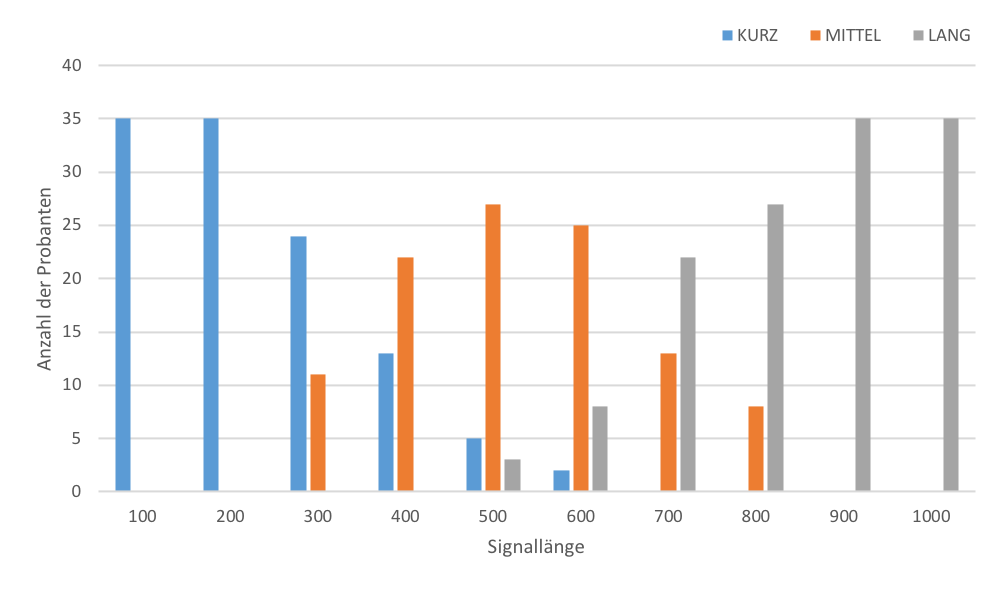
\includegraphics[width=\textwidth]{pics/analyse/Initialisierung.png}
	\caption{}
	\label{fig:Initialisierung}
\end{figure}

F{\"u}r die Bestimmung der Grenzen von Kurz, Mittel und Lang hat der Benutzer 10 Signale zu der jeweiligen Kategorie einordnen sollen. 
Da man bei 16\% der Probanden bei diesem Schritt keine eindeutigen Grenzen bestimmen konnte, musste der Schritt ein weiteres mal wiederholt werden. Die Auswertung der {\"u}bertragung hat ergeben, dass es im Durschnitt 300ms gedauert hat, bis das Signal {\"u}bertragen worden ist.

Obwohl die 10 normalverteilten Signale in zuf{\"a}lliger Reihenfolge abgespielt wurden, wurde bei 84\% aller Probanden die zehn Signale so bewertet, dass zuerst alle Kurz, gefolgt von nur Mittel und anschlie{\ss}end nur Lang bewertet wurden. 
Die restlichen Probanden haben an den Grenzen der Signaltypen nur \textit{Kurz} und \textit{Mittel} oder \textit{Mittel} und \textit{Lang} vertauscht.
%von Kurz und Mittel oder Mittel und Lang vertauscht gehabt.

%Au{\ss}erdem ist bei 84\% aller Probanden die Zuordnung der Kategorie zu den Signalen so bewertet worden, dass zuerst eine Anzahl von Signalen als Kurz, gefolgt von einer weiteren Anzahl als Mittel und schlie{\ss}lich der Rest als Lang erkannt worden ist.
%dass zuerst alle Signale als Kurz, gefolgt von nur Signale als Mittel und schlie{\ss}lich nur Signale vom Langen . 

%Die restlichen 16\% der Probanden haben an den Grenzen der Signaltypen nur ein Signal vom Kurz und Mittel oder Mittel und Lang vertauscht gehabt.

In der Auswertung \autoref{fig:Initialisierung} haben sich drei Normalverteilungen gebildet. 
Daraus kann man entnehmen, dass Werte 100ms und  200 ms eindeutig als Kurz, sowie auch Werte 900ms und 1000ms als Lang erkannt worden sind. 
Einen eindeutigen Hochpunkt f{\"u}r Mittel hat man bei dem Wert von 500ms, dennoch gab es einige Probanden f{\"u}r die dieser Wert noch als Kurz oder Lang empfunden wurde. 

Aus dem Diagramm kann man sehr sch{\"o}n erkennen, dass man eine Personalisierung von Vibrationen ben{\"o}tigen k{\"o}nnte, da man au{\ss}er den R{\"a}ndern keine eindeutige Zuweisung von \textit{Kurz}, \textit{Mittel} oder \textit{Lang} unter allen Probanden bestimmen konnte. 
Man kann zwar im Vorfeld Werte f{\"u}r Signale definieren, wie es derzeitig einige Firmen machen, diese Werte k{\"o}nnten jedoch von Personen unterschiedlich wahrgenommen werden.
%Aus dem Diagramm kann man sehr sch{\"o}n erkennen, dass man Werte zwar im Vorfeld selbst definieren kann, diese Werte k{\"o}nnten unter verschiedenen Probanden jedoch anders wahrgenommen werden und es wei{\ss}t darauf hin, dass man sehr wohl eine Personalisierung von Vibrationen ben{\"o}tigen k{\"o}nnte. 

%% ==============================
\subsection{Auswertung der Iterationen des Algorithmus}
%% ==============================


\paragraph{Verlauf der Grenzen}

\begin{figure}[htbp] 
	   \centering
   	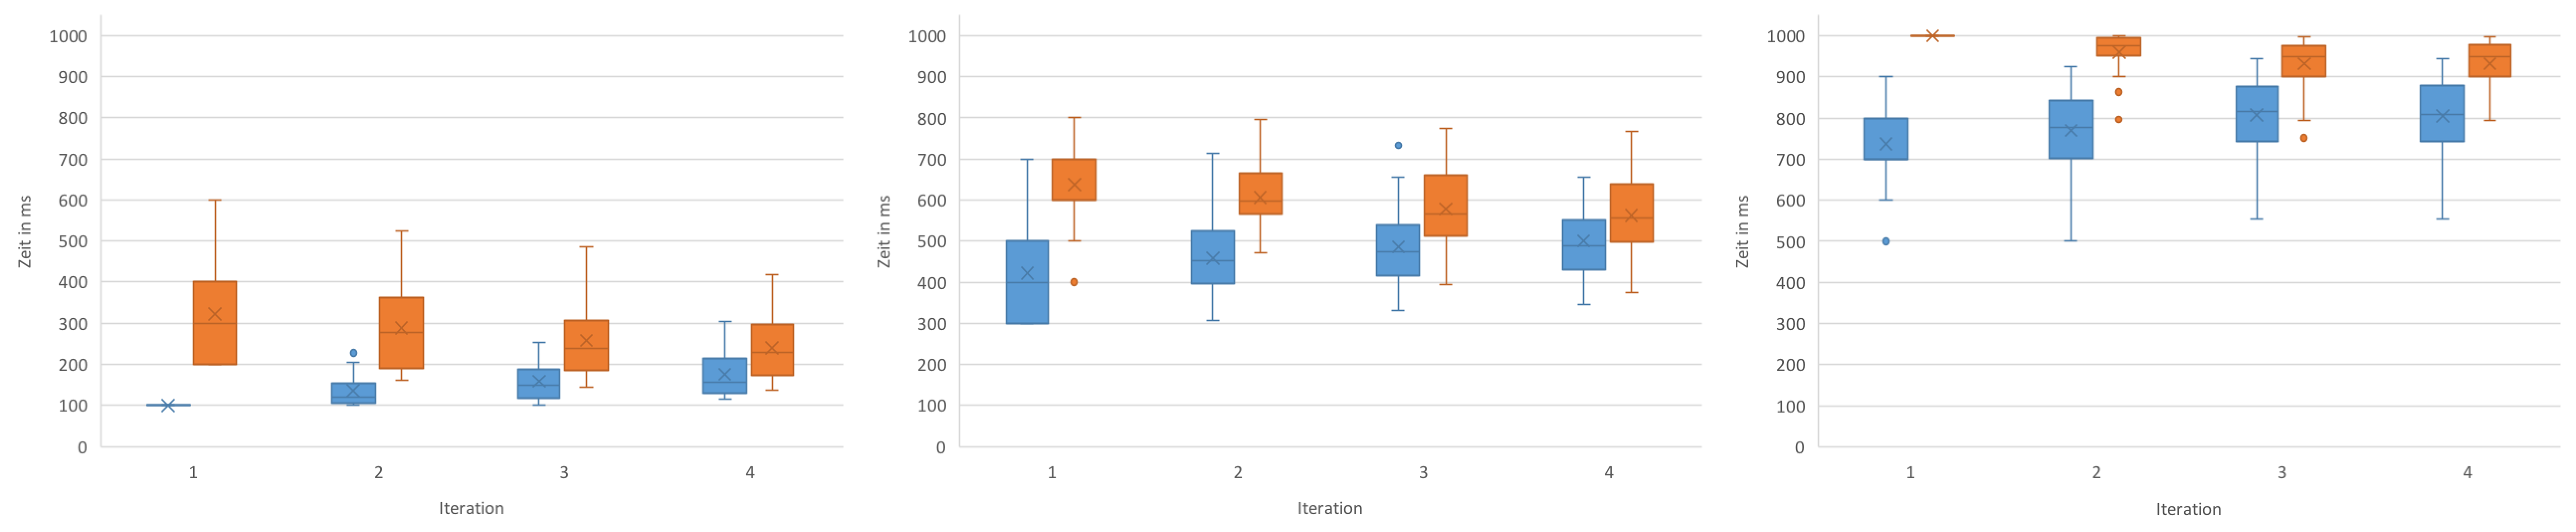
\includegraphics[width=\textwidth]{pics/analyse/algo/MinMax/MinMaxFinal.png}
	\caption{Darstellung des Minimum (in blau) und Maximum (in rot) im Verlauf der 4 Iterationen des Algorithmus. Das erste Bild zeit Kurz, gefolgt von Mittel und Lang.}
	\label{fig:MinMaxSignale}
\end{figure}

Der Algorithmus wurde insgesamt vier mal ausgef{\"u}hrt, anschlie{\ss}end wurde aus der letzten Population der personalisierte Wert gemittelt. 

\paragraph{Kurz}
Eine der gr{\"o}{\ss}ten Ver{\"a}nderungen im Diagramm \autoref{MinMaxSignale} gibt es bei \textbf{Kurz}; die oberste Grenze vom Maximum ist nach vier Iterationen von 600ms auf 415ms gesunken. 
Die obere Grenze des Minimum ist von 100ms auf 300ms gestiegen. 
%Der Bereich verkleinert insgesamt das Intervall um 44\% von 100 bis 600ms auf 140 bis 420 ms. 
Der Median von den Maximum und Minimum konvergieren in die gleiche Richtung. 
Nach vier Iterationen ist der Median vom Minimum um 80ms nach oben und der Median von dem Maximum auch um 80ms nach unten gewandert. 
Das Minimum und Maximum {\"u}berschneidet sich in der 2. Iteration nur minimal. 
In der 4. Iteration {\"u}berschneiden sich Minimum und Maximum um 150ms. 
Das 50\% Quartil vom Minimum w{\"a}chst um bis zu 100ms, wobei das 50\% Quartil beim Maximum von einem 200ms Intervall auf ein 120ms Intervall verkleinert. 
Das gesamte Intervall von \textit{Kurz} verkleinert sich insgesamt um 44\% von 100-600ms auf 140-420ms, somit ist das die gr{\"o}{\ss}te Ver{\"a}nderung unter allen Intervallen.



\paragraph{Mittel}
In der ersten Iteration besitzt man schon {\"u}berschneidungen des Minimum und Maximum. 
Von der ersten zur zweiter Iteration verschieben sich die Grenzen des Minimum um ca. 10 ms nach oben, diese werden im Verlauf der Iteration minimal kleiner.  
Die Grenzen des Maximums hingegen werden gr{\"o}{\ss}er und verschieben sich anschlie{\ss}end minimal nach unten. 
Das 50\% Quartil verkleinert sich um 40\% sich beim Minimum von einem 200ms Intervall auf ein 120ms Intervall und verschiebt sich anschlie{\ss}end im Verlauf der folgenden Iterationen nur nach oben. 
Bei \textit{Mittel} habt sich das gesamt Intervall um 16\% von 300-800ms auf 345-766ms verkleinert.


\paragraph{Lang}
Die meisten Ausrei{\ss}er sind in bei Lang vertreten, hier hat man in der zweiten Iteration schon ein Maximum von 1000ms auf unter 800ms und 880ms erhalten, das ist eine {\"a}nderung eines Maximums um 200ms nach nur einer Iteration bei einem Probanden.
Die 50\% Quartile des Maximums werden Minimal gr{\"o}{\ss}er und wachsen nach unten.
Das 50\% Quartile des Minimums werden die kurzzeitig gr{\"o}{\ss}er, minimiert sich minimal wieder im Verlauf.
Die Grenzen des gesamten Intervalls von \textit{Lang} haben sich um 11\% von 500-1000ms auf 555-997ms minimiert.
Zwischen der 3. und 4. Iteration bei \textit{Lang} ist es das einzige mal vorgekommen, dass zwischen zwei Itterationen bis auf 3ms keine Unterschiede erkennbar sind.
Das w{\"u}rde bedeuten, dass nach der 3. Generation f{\"u}r die Probanden schon ein sehr gut unterscheidbares Ergebnis vorhanden gewesen ist.
% {\"a}ndern sich aber wieder auf mit dem Ausrei{\ss}er der ersten Iteration auf das gleiche Intervall und verschieben sich pro Iteration leicht nach oben.

%\\

Unter den Signaltypen {\"u}berschneiden sich die Iterationen die Grenzen selbst zwischen den Iterationen selbst. 
Diese {\"U}berschneidungen verringern sich nach den 4 Iterationen.

Das Minimum steigt stetig und das Maximum verringert sich. 
Denn genau diesen Effekt wollte man auch erzielen, dass der Benutzer zu seinen personalisierten Wert konvergiert.
Bei Kurz und Mittel {\"u}berschneiden sich die 50\% Quartile. 
Bei Lang {\"u}berschneiden diese in keiner Iteration.

Schlussfolgernd kann man sagen, dass die man anhand der 50\% Quartile vom Maximum und Minimum aller Probanden einen Kurzes Signal in dem Bereich von 130ms bis 300ms, ein Mittleres Signal zwischen 430ms und 640ms und ein Langes Signal zwischen 740ms und 980ms die gebildet haben. 




\paragraph{Grenzen nach dem Algorithmus}

\begin{figure}[htbp] 
            \centering
   	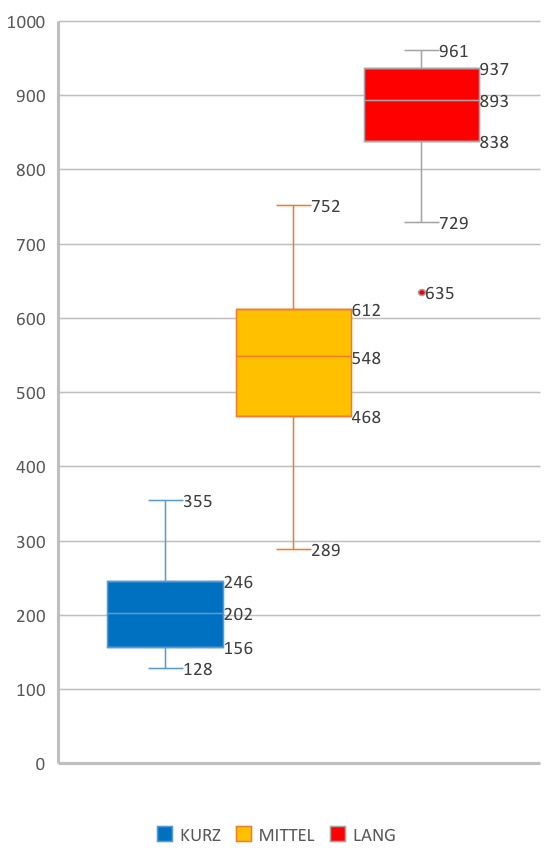
\includegraphics[width=\textwidth]{pics/analyse/algo/MinMax/GrenzenNachAlgo.png}
	\caption{Nach der Vierten Iteration gemittelte personalisierte Werte in ms}
	\label{fig:GrenzenNachAlgo}
\end{figure}

In dem Diagramm \autoref{fig:GrenzenNachAlgo} sind alle gemittelten personalisierten Werte nach der vierten Iteration abgebildet. 
Daraus l{\"a}sst sich ableiten, dass zwischen den Signaltypen von \textit{Kurz}, \textit{Mittel} und \textit{Lang} sich die Grenzen {\"u}berschneiden und man somit sagen kann, dass man diese Bereiche auf f{\"u}r vordefinierte Signale meiden sollte. 
Die Grenzen {\"u}berschneiden zwischen \textit{Kurz} und \textit{Mittel} von 289-355ms und zwischen \textit{Mittel} und \textit{Lang} von 729-752ms.
F{\"u}r die einzelnen Signaltypen hat sich der Median f{\"u}r \textit{Kurz} bei 202ms, f{\"u}r \textit{Mittel} bei 548ms und \textit{Lang} bei 893ms bestimmen k{\"o}nnen.
Die oberen 25\% von \textit{Lang} und die unteren 25\% von \textit{Kurz} weisen nur eine minimale Abweichung auf. 
Im Gegensatz dazu gibt es eine Abweichung von genau 109ms bei den oberen 25\% von \textit{Kurz} und den unteren 25\% von \textit{Lang}.
Es gibt einen Ausrei{\ss}er bei \textit{Lang} mit einem Wert von 635ms, dabei handelt es sich nicht um keinen Fehler, sondern einen Probanden der genau dies f{\"u}r sich als personalisierten Wert bestimmt hat.
Im Vergleich der inneren 50\% von den jeweiligen Signaltypen wei{\ss}t \textit{Kurz} einen Intervall von 90 ms und \textit{Lang} einen Intervall von 99ms auf, wobei \textit{Mittel} diesen Wert von 144 ms am gr{\"o}{\ss}ten Bereich ist und um nahezu 50ms gr{\"o}{\ss}er als Kurz und Lang ist. 


\paragraph{Stimmung im Verlauf des Algorithmus}

\begin{figure}[htbp] 
            \centering
   	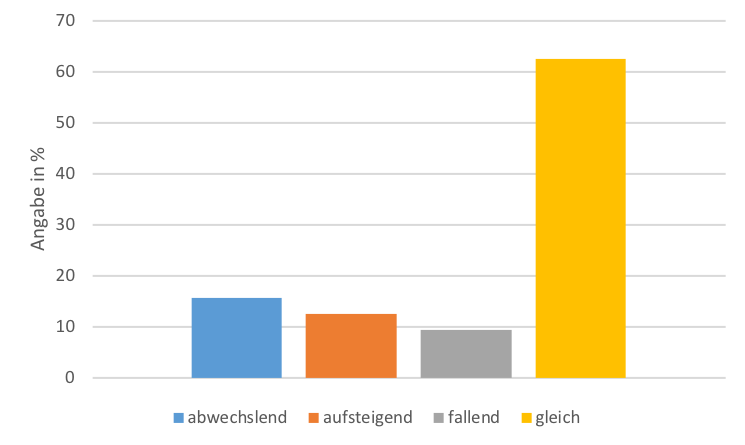
\includegraphics[width=\textwidth]{pics/analyse/person/Stimmung.png}
	\caption{Bewertung der Stimmung}
	\label{fig:Stimmung}
\end{figure}

Nach jeder Iteration wurden die Benutzer gefragt, wie Ihre Stimmung \autoref{fig:Stimmung} aktuell sei. 
Dabei hat es bei 62\% aller Probanden keine {\"A}nderung der Stimmung gegeben. 
Diese Probanden hatten Ihre Stimmung mit \textit{Gut} oder \textit{Sehr gut} bewertet gehabt. 
Im Gegensatz dazu hat sich die Stimmung bei 16\% der Probanden entweder zwischen \textbf{Gut} und \textbf{Sehr gut} oder \textbf{Gut} und \textbf{OK} abgewechselt. 
Des Weiteren gab es bei 13\% der Probanden eine aufsteigende Stimmung und bei den restlichen 9\% ist die Stimmung pro Iteration gefallen.

Somit kann man feststellen, dass die Anzahl von vier Iterationen keinen wirklichen Einfluss auf die Stimmung des Benutzers ausgewirkt hat.

% die ben{\"o}tigt wurde um den Algorithmus auszuf{\"u}hren, sich nicht auf die Stimmung Stimmung sich nicht  ausgewirkt hat. 

\paragraph{Replays eines Signals}

\begin{figure}[htbp] 
            \centering
   	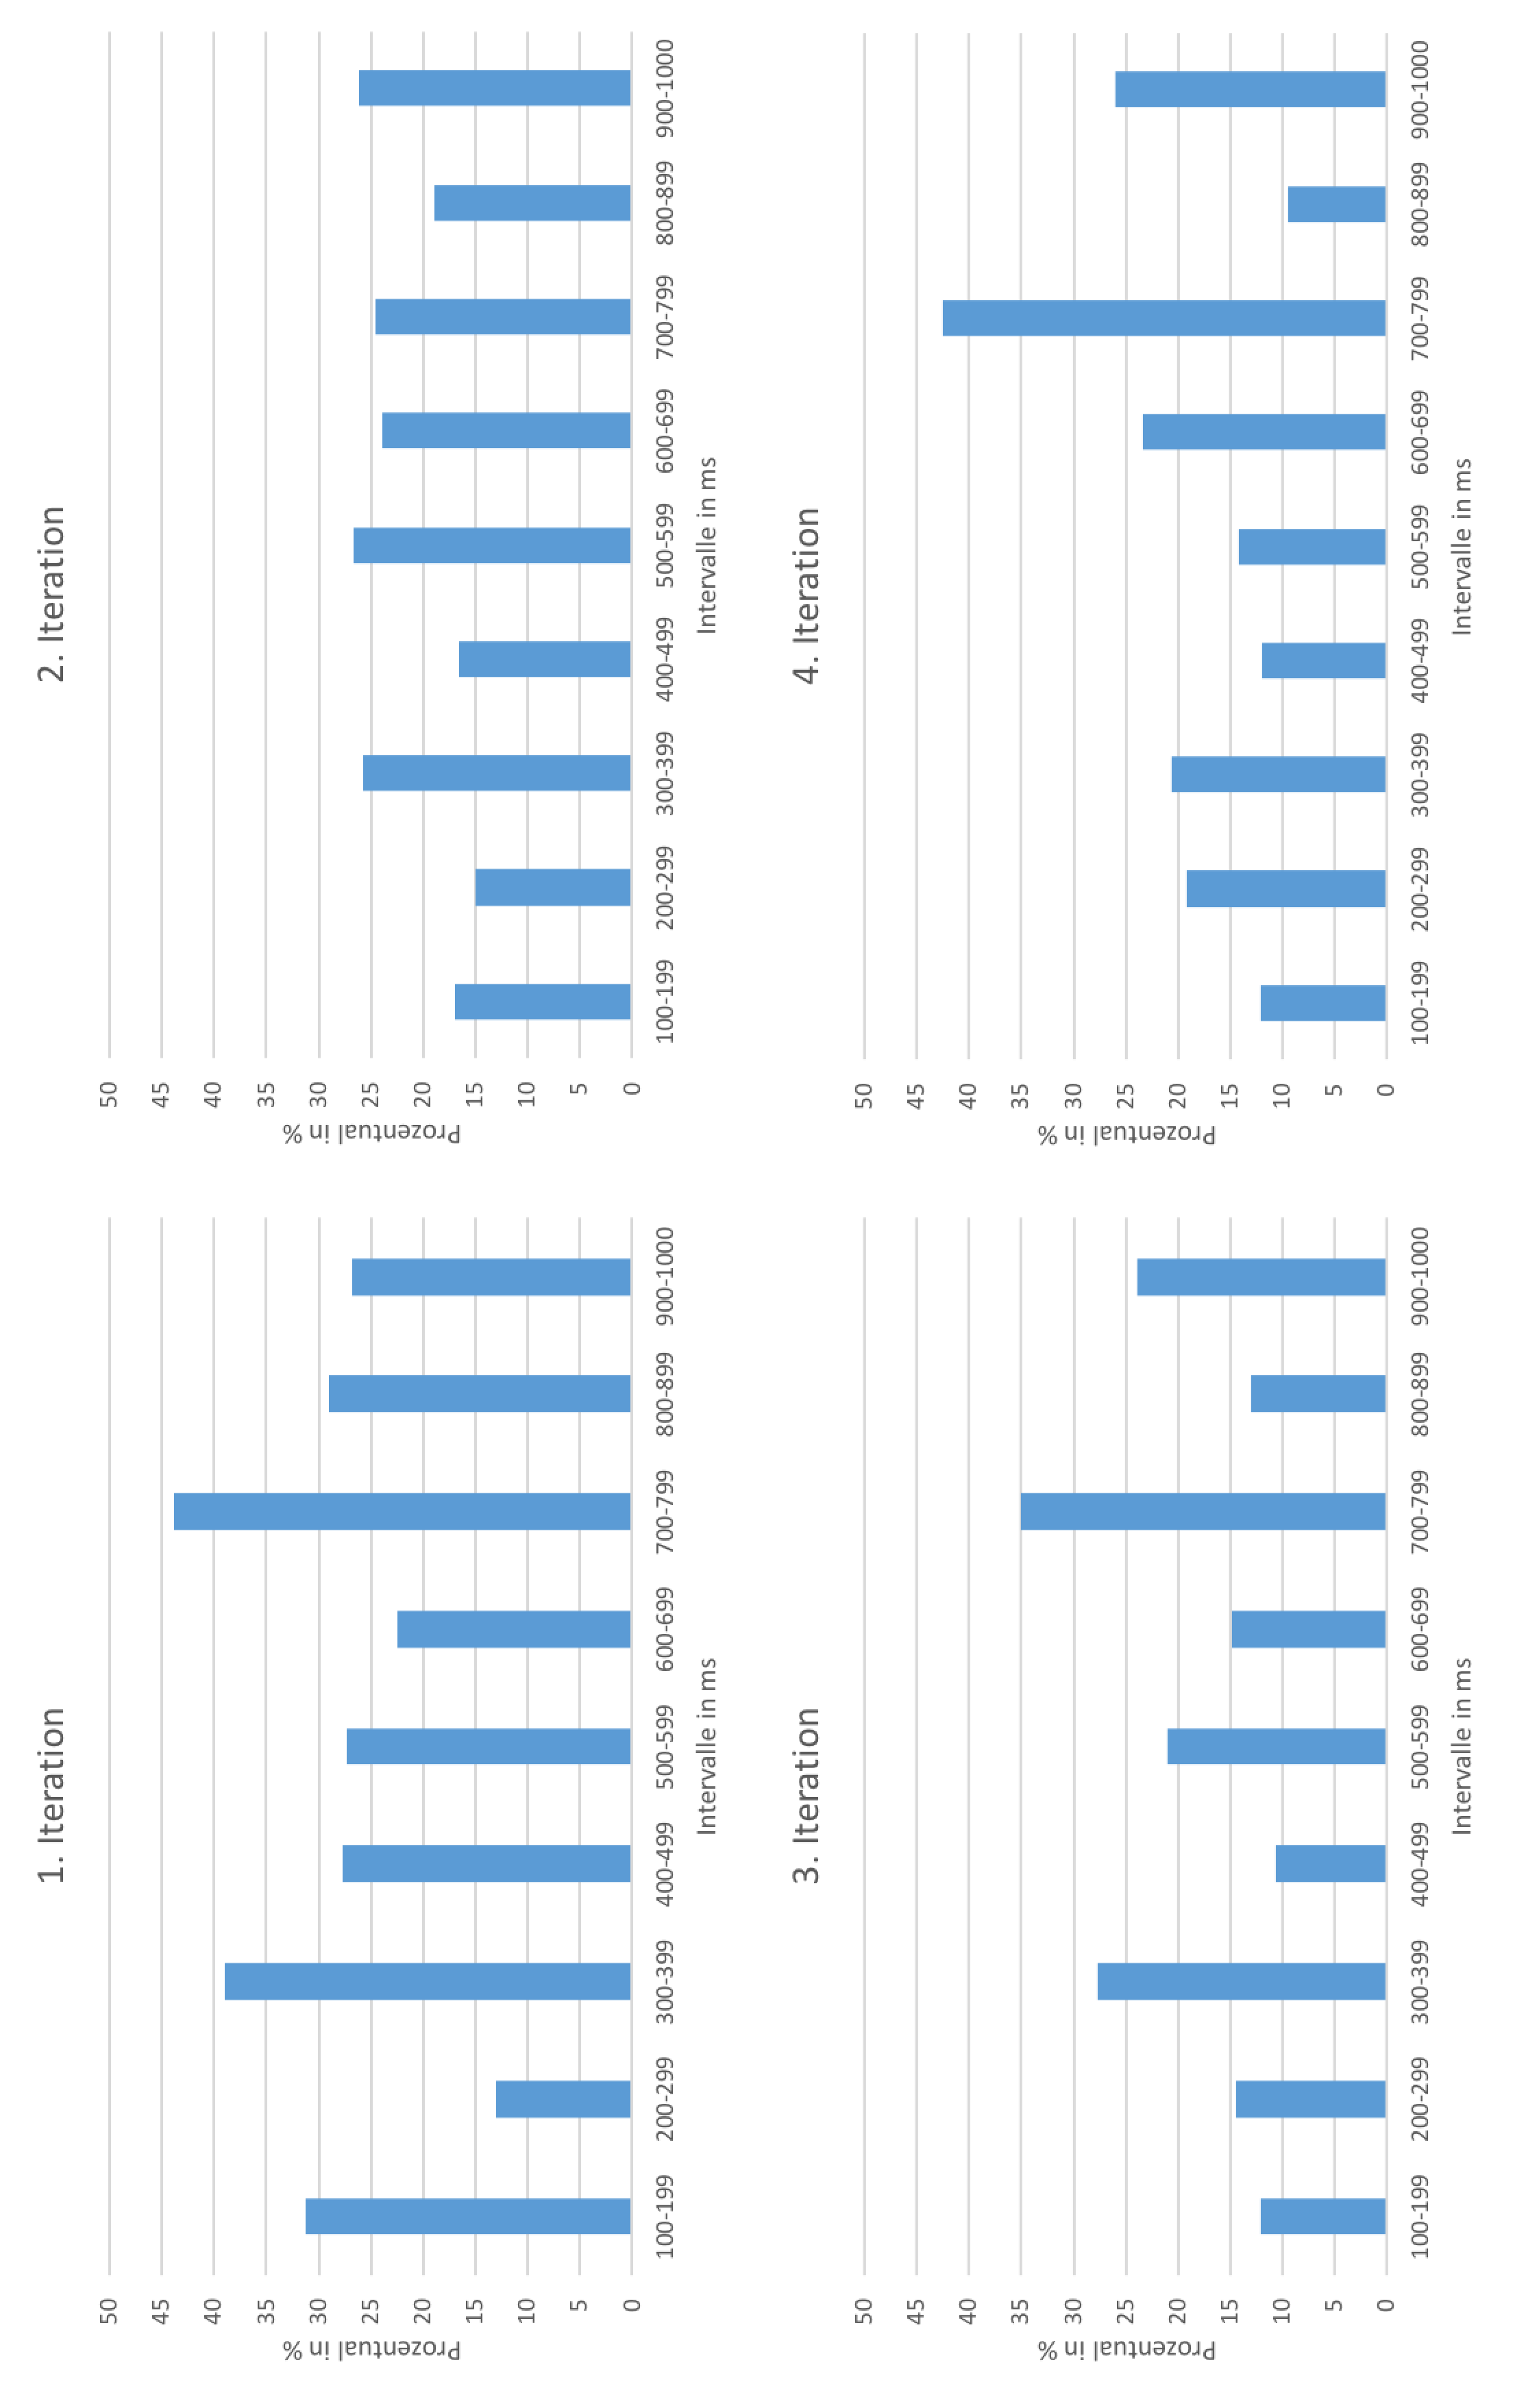
\includegraphics[width=\textwidth]{pics/analyse/algo/Replay/ReplayFinal290.png}
	\caption{Anzahl der Replays innerhalb von Zeitintervallen {\"u}ber dem Verlauf des Algorithmus}
	\label{fig:ReplayFinal290}
\end{figure}

Man hat dem Probanden die M{\"o}glichkeit geboten, ein Signal wiederholen zu d{\"u}rfen. 
Im Verlauf des Algorithmus wollte man herausfinden wie oft unter allen Probanden auf Replay f{\"u}r ein bestimmtes Intervall Replay gedr{\"u}ckt wurde \autoref{fig:ReplayFinal290}. 
%Die Anzahl der wie oft auf Replay gedr{\"u}ckt wurde 

In der ersten Iteration haben 44\% der Probanden in dem Intervall von 700-799ms die gr{\"o}{\ss}ten Schwierigkeiten gehabt ein Signal zuzuordnen und sich das Signal erneut abgespielt. 
Der Bereich, der am wenigsten wiederholt abgespielt werden musste war 200-299ms. 
Die Restlichen Intervalle der ersten Iteration wurden mit einem Mittelwert von 32\% erneut abgespielt.

In der zweiten Iteration hat sich die Anzahl der Replays um einiges verringert, hier war der Mittelwert insgesamt bei 22\%, das Minimum war bei 200-299ms im Wert von 15\% und das Maximum bei 500-599ms mit 27\%.  
Die dritte Iteration hat eine Verbesserung bei allen nahezu allen Werten gehabt, bis auf das Intervall von 700-799ms was auf 35\% angestiegen ist; insgesamt ist der Mittelwert in dieser Iteration bei 19\%. 

Selbst in der letzten Iteration hat sich ein globales Minimum unter allen Iterationen bei 800-899ms von 9,5\% gebildet. Der globale Maximum war bei 700-799ms in der ersten Iteration mit 43\%, ist aber auch in der vierten Iteration, trotz Verbesserungen zwischen durch das Maximum mit 42,5\%. 

Man kann daraus erkennen, dass die Probanden genau an dem Bereich von Kurz zu Mittel, was sich in der 4. Iteration bei 200-399ms bewegt, und Mittel zu Lang, dass zwischen 600-799ms liegt, am meisten den Replay Knopf gedr{\"u}ckt haben. 
Ein viertel aller Probanden haben bei 900-1000ms in jeder Iteration das Signal erneut abgespielt. 
Jedoch kann man in der vierten Iteration sehr gut erkennen, dass die Signale mit den Werten 100-199ms, 400-599ms und 800-899ms am geringsten erneut abgespielt werden mussten.
Im Durchschnitt wurde, der Replay Button 1,7mal gedr{\"u}ckt, wenn man ein Signal erneut abgespielt haben wollte. 
Dabei war das Minimum einmal und das Maximum neun mal, dass man das Signal erneut abgespielt hat.

\paragraph{Mittelwert}
Beim Verlauf des Algorithmus konnte man feststellen, dass zwischen der ersten und der letzten Iteration unter allen Probanden der Mittelwert sich wie im folgenden Verhalten hat. 
\textit{Kurz} hatte eine durchschnittliche Abweigung von 10,11\% bei einem Minimum von 1\% und einem Maximum von 23\%. 
Weiterhin habe sich der Mittelwert bei den beiden Signaltypen \textit{Miitel} und \textit{Lang} von der ersten zur letzten Iteration im Durchschnitt nur um 3,34\% ver{\"a}ndert.
Dabei war das Minimum bei 0,09\% und ein Maximum bei 9,9\% f{\"u}r \textit{Mittel} sowie ein Minimum von 0,06\% und ein Maximum von 15,33\% f{\"u}r \textit{Lang} vorhanden.

\paragraph{Beantwortung der Fragen}
\begin{figure}[htbp] 
            \centering
   	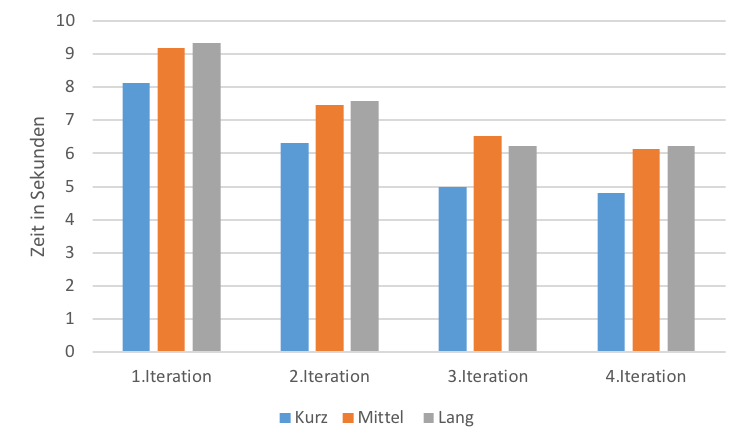
\includegraphics[width=\textwidth]{pics/analyse/algo/ZeitDurchschnitt.png}
	\caption{Durchschnittlich ben{\"o}tigte Zeit der Probanden, um die drei Fragen des Algorithmus zu bewerten.}
	\label{fig:ZeitDurchschnitt}
\end{figure}
Im Verlauf des Algorithmus hat man auch die Zeit \autoref{fig:ZeitDurchschnitt}, die ben{\"o}tigt wurde um die Fragen f{\"u}r ein Signal zu beantworten, gespcierht. 
Daraus hat sich ergeben, dass \textit{Kurz} in jeder Iteration um einer ganzen Sekunde schneller beantwortet wurde. 
F{\"u}r \textit{Mittel} und \textit{Lang} hat man im Durchschnitt immer gleich viel Zeit ben{\"o}tigt.
Nach der dritten Iteration ist der Wert f{\"u}r alle drei Signaltypen nahezu konstant geblieben, desweiteren hat sich bis zur dritten Iteration bei allen Signaltypen der Wer um drei Sekunden verringert. 
Daraus l{\"a}sst sich ableite, dass die Probanden sich an die Signale gew{\"o}hnt haben und die drei Fragen schneller beantworten konnten.

\paragraph{Verlauf der Werte}
\begin{figure}[htbp] 
            \centering
   	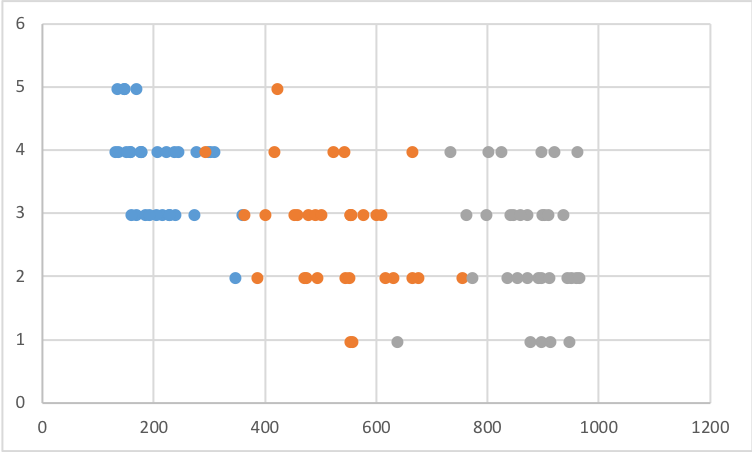
\includegraphics[width=\textwidth]{pics/analyse/algo/ergebnisnachAlgo.png}
	\caption{Personalisierte Werte der einzelnen Probanden, die in dem Diagramm der St{\"a}rke {\"u}ber die Zeit dargestellt werden.}
	\label{fig:ergebnisNachAlgo}
\end{figure}

Anhand des Diagramms \autoref{fig:ergebnisNachAlgo} kann man erkennen, dass die meisten Probanden ein st{\"a}rkeres \textit{Kurz} Signal sowie ein schw{\"a}cheres \textit{Lang} Signal bevorzugt haben. F{\"u}r das Signal \textit{Mittel} hat man sich jedoch in dem mittleren St{\"a}rkebereich befunden.

\begin{figure}[htbp] 
            \centering
   	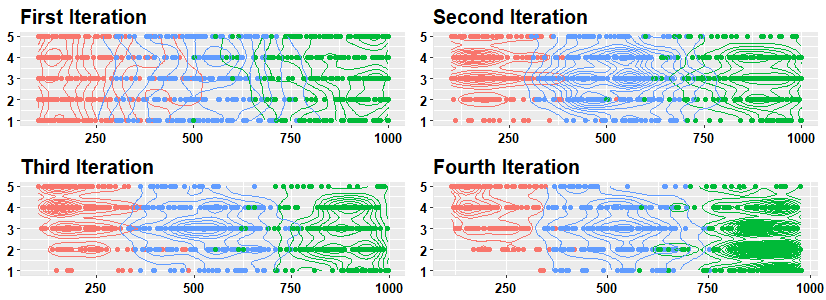
\includegraphics[width=\textwidth]{pics/analyse/algo/gruppierung.png}
	\caption{Darstellung der St{\"a}rke zu der jeweiligen Signall{\"a}nge {\"u}ber dem Verlauf des Algorithmus. Dabei bildet rot \textit{Kurz}, blau \textit{Mittel} und gr{\"u}n \textit{Lang} ab.}
	\label{fig:gruppierung}
\end{figure}

In der ersten Itteration \autoref{fig:gruppierung} sieht man sehr sch{\"o}n, wie es noch keine wirklliche Unterteilung existiert, es gibt die Bereiche bis 250ms in denen sich das Signal \textit{Kurz} befindet und von 800-1000ms auch \textit{Lang}, aber es gab {\"u}berschneidungen in den Bereich von \textit{Mittel} mit den anderen beiden Signaltypen. 
Anhand der zweiten Iteration haben sich schon leichte Cluster gebildet, bei denen es dennoch Ausrei{\ss}er von Kurz und Mittel an den Werten nahe 500ms existieren. 
Bis zur vierten Iteration verdichten sich die Signale von \textit{Kurz} in dem oberen linken Bereich, das bedeutet, dass man f{\"u}r Signale vom Typ \textit{Kurz} eher st{\"a}rkere Signale bevorzugt hat. 
Die Signale des Typs \textit{Mittel} haben im Verlauf des Algorithmus genau in der Mitte bei dem Wert 500ms und der mittleren St{\"a}rkestufe eine Hochpunkt gebildet. 
Desweiteren hat sich das Signaltyp \textit{Lang} in den St{\"a}rkestufen eins (f{\"u}r sehr schwach) bis drei (f{\"u}r o.k.) einzelne Cluster gebildet. 
Wohingegen bei \textit{Kurz} und \textit{Mittel} sich ein Hochpunkt gebildet haben, hat sich bei \textit{Lang} f{\"u}r die St{\"a}rkestufen eins (f{\"u}r sehr schwach) bis drei (f{\"u}r o.k.) jeweils ein Cluster gebildet.

Man kann zweifellos erkennen, dass wenn man noch weitere Iterationen ausgef{\"u}hrt h{\"a}tte, w{\"u}rde sich das Ergebnis weiter in einem Punkt verdichten. 

%H{\"a}tte man noch mehr Iterationen des Algorithmus ausgef{\"u}hrt, w{\"a}re es zweifellos, dass sich das Ergebnis weiter in einem Punkt verdichten w{\"u}rden. 


\paragraph{MUSTER}

\begin{table}[]
\centering
\caption{Durchschnittliche Genauigkeit zur Erkennung eines Signals der Probanden {\"u}ber die Kategorien (Angaben in \%)}
\label{MusterGenauigkeit}
\begin{tabular}{llllll|l}
\hline
\multicolumn{3}{l}{Genetisch} & \multicolumn{3}{l|}{Generisch} & Kategorie      \\ \hline
3er    & 4er    & 5er   & 3er    & 4er    & 5er   &                             \\ \hline
81     & 77     & 75    & 76     & 69     & 66    & {\"u}ber alle Probanden         \\ \hline
76     & 71     & 74    & 75     & 67     & 63    & weiblich                    \\
83     & 79     & 77    & 80     & 74     & 71    & m{\"a}nnlich                    \\ \hline
80     & 74     & 77    & 79     & 74     & 71    & musikalisch                 \\
80     & 75     & 72    & 77     & 69     & 66    & nicht musikalisch           \\ \hline
81     & 76     & 75    & 78     & 72     & 70    & spielen Spiele              \\
75     & 70     & 70    & 74     & 63     & 58    & spielen keine Spiele        \\ \hline
86     & 84     & 80    & 83     & 79     & 75    & nutzten Smartwatch          \\
78     & 72     & 72    & 76     & 68     & 66    & nutzten keine Smartwatch    \\ \hline
83     & 78     & 73    & 80     & 70     & 67    & nutzten Taktiles Ger{\"a}t      \\
76     & 72     & 75    & 75     & 70     & 69    & nutzten kein Taktiles Ger{\"a}t
\end{tabular}
\end{table}

Die Tabelle \autoref{MusterGenauigkeit} beschreibt, wie genau die Probanden ein Signal aus den Mustern erkennen konnten, man hat die generischen Muster mit den genetischen Mustern verglichen, sowie f{\"u}r jede Gruppierung von Probanden die Auswertung neu bestimmt. 
%Die Tabelle \autoref{MusterGenauigkeit} beschreibt, wie genau die Probanden ein Muster ohne Fehler erkennen konnten, man hat die generischen Muster mit den genetischen Mustern verglichen, sowie f{\"u}r jede Gruppierung von Probanden die Auswertung neu bestimmt. 
%Dabei hat man in den jeweiligen Kategorien nach den gelisteten Kategorien die Genauigkeit gruppiert.

Laut der Tabelle kann man feststellen, dass die Probanden die keine Computerspiele spielen, die einzelnen Signale der generischen f{\"u}nfer Muster nur zu 58\% richtig erkannt haben. Dieser Wert ist das Globale Minimum unter allen Gruppierungen der Probanden.
Bei den Probanden, die schon einmal eine Smartwatch nutzten, haben bei den genetischen dreier Mustern ein einzelnes Signal mit 86\% Wahrscheinlichkeit richtig erkannt, der auch als globales Maximum unter allen Probanden-Gruppen existiert.

%Das Globale Maximum ein Signal richtig zu erkennen, war bei den genetischen Mustern mit drei Signalen, bei einem Wert von 86\% durchschnittlicher Genauigkeit bei Probanden, die schon mal eine Smartwatch benutzt hatten. 
%Das Globale Maximum war bei den genetischen Mustern mit drei Signalen bei einem Wert von 86\% durchschnittlicher Genauigkeit bei Probanden, die schon mal eine Smartwatch benutzt hatten. 
%Das Globale Minimum war bei der Gruppe an Probanden die keine Computerspiele spielen und zwar mit der Genauigkeit von 58\% bei generischen Mustern mit 5 Signalen.

Unter den vorliedenden Ergebnissen, haben die m{\"a}nnlichen Probanden im Vergleich zu den weiblichen Probanden die einzelnen Signale unter allen Muster-Typen besser erkannt.
%Unter den vorliegenden Ergebnissen, waren die m{\"a}nnlichen Probanden bei der Erkennung von komplett richtigen Mustern im Durchschnitt immer um einige Prozent besser.
Die musikalischen und nicht musikalischen Probanden erkennen bei den dreier Mustern die Signale gleich gut, wobei bei den vierer und f{\"u}nfer Muster die musikalischen Probanden bis zu 5\% besser waren.
Bei den dreier Mustern k{\"o}nnen die musikalischen im Vergleich zu nicht musikalischen Probanden die Signale gleich gut erkennen, jedoch zeigen die musikalichen Probanden bei vierer und f{\"u}nfer Muster eine Verbesserung bis zu 5\%.
%Unter der Kategorie "`musikalisch"' kann man nachvolzeihen, dass bei den dreier Mustern die Signale gleichgut erkannt worden sind. 
%Bei den Musikalischen Probanden sind bei den genetischen dreier Mustern gleich gut wie die nicht musikalischen Probanden. 
%Bei den vierer und f{\"u}nfer Signalen waren die musikalischen Probanden jedoch um bis zu 5\% besser.
Allgemein k{\"o}nnen die gelegendlich Computerspiele spielenden Probande im Gegensatz zu nicht-Spielern alle abgespielten Signale der Muster-Typen besser zuweisen. Wenn wir ins Detail gehen, liegt bei den generischen f{\"u}nfer Muster die Abweichung von 12\%.
%Die Probanden die gelegendlich Computerspiele spielen, haben die Signale aller Muster-Typen besser erkannt, als die Probanden die keine Computerspiele gespielt haben, hier lag der gr{\"o}{\ss}te Unterschied n{\"a}mlich bei den generischen f{\"u}nfer Muster, die eine Abweichung von 12\% aufweisen.
%Die Probanden die gelegendlich Computerspiele spielen haben die Muster im Durchschnitt genauer erkannt als die Probanden die keine Computer spiele gespielt haben, hier lag der gr{\"o}{\ss}te Unterschied n{\"a}mlich bei den generischen f{\"u}nfer Muster, die eine Abweichung von 13 \% aufweisen.
Dasselbe Ergebnis, n{\"a}mlich 12\% Unterschied kommt bei Probanden vor, die schon mal eine Smartwatch getragen haben.
%Das selbe gilt f{\"u}r die Probanden, die schon mal eine Smartwatch benutzt haben, hier lag der Unterschied bei 12 \%.

Bei der letzten Gruppe wird es interessant, denn hier haben genau 50\% der Probanden schon mal ein Taktiles Ger{\"a}t verwendet. 
Dabei wurde um 8\% der Signale der genetischen dreier Muster sowie um 4\% der generischen Muster von den Teilnehmern, die Erfahrung mit den taktilen Ger{\"a}ten hatten, besser erkannt.
%Dabei wurden die Signale der genetischen dreier Muster um 8\% und bei den generischen Mustern um 4\% besser erkannt.
%Diese waren bei den genetischen dreier Mustern um 8\% besser erkannt und die generischen um nur 4\%. 
Bei den Signalen der f{\"u}nfer Muster haben die Probanden, die schon einmal ein Taktiles Ger{\"a}t verwendet haben, die Signale um 2\% besser erkannt.
%Bei den f{\"u}nfer Mustern haben Probanden, die schon mal ein Taktiles Ger{\"a}t verwendet haben die Signale um 2\% besser erkannt. 

Im Vergleich zu den generischen Muster wurden die Signale der genetischen Muster {\"o}fter richtig zuge{\"o}rdnet. 
Die Genauigkeit erreichte sogar bei dem genetischen dreier Muster bis zu 82\%. 
Somit ist es um 5\% besser als der Wert von der generischen dreier Muster.
%Im Vergleich der genetischen und generischen Muster aller Probanden, wurden die Genetischen Signale eindeutig {\"o}fter richtig erkannt als die generischen Werte. 
%Die genetischen dreier Muster wurden die Signale mit 82\% um 5\% besser erkannt als die generischen dreier Muster. 
Obwohl der Prozenzsatz bei den vierer Mustern ingesamt gesunken ist, gewinnt jedoch der Unterschied an Ausdehnung.
Hier erh{\"o}ht sich das Optimierungspotenzial bei genetischen vierer Mustern um 8\%.
%Bei den vierer Mustern ist der Prozenzsatz insgesamt weiter herunter gegangen, jedoch ist der Unterschied gr{\"o}{\ss}er geworden und zwar ist es auf 77\% bei den genetischen vierer Mustern im Vergleich eine Verbesserung von 8\% zum generischen. 
Generell wurden 75\% der Signale bei den genetischen f{\"u}nfer Mustern korrekt erkannt und somit wird nur zwei drittel der Signale von den generischen f{\"u}nfer Mustern als richtig empfunden.
%Bei den f{\"u}nfer Signalen wurden drei von vier Signale (75\%) korrekt erkannt. 
%Bei den generischen f{\"u}nfer Mustern wurden nur zwei von drei Signalen richtig erkannt. \\

%Unter Betrachtung der genetischen und generischen Muster, gibt es bei den dreier Mustern eine minimale Abweichung von 0\% bis zu einem Maximum von 5\%, in denen die genetischen Muster besser erkannt worden sind als die generischen. 
%Bei den 4er Muster sieht es {\"a}hnlich aus, mit einem Minimum von 0\% und einem Maximum von 8\% Abweichung. 
%Bei den 5er Mustern hat man eine Abweichung von 4\% bis zu 12\%. 


%Die Auswertung meiner Daten haben ergeben, dass musikalische Probanden 


\begin{figure}[htbp] 
	\centering
	\begin{minipage}[t]{0.4\textwidth}
		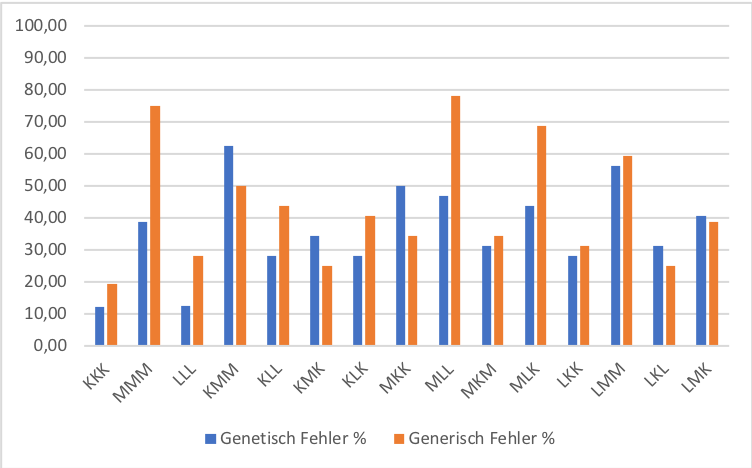
\includegraphics[width=\textwidth]{pics/analyse/algo/ohneFehler/Fehler3.png}
	\end{minipage}
	\begin{minipage}[t]{0.4\textwidth}
		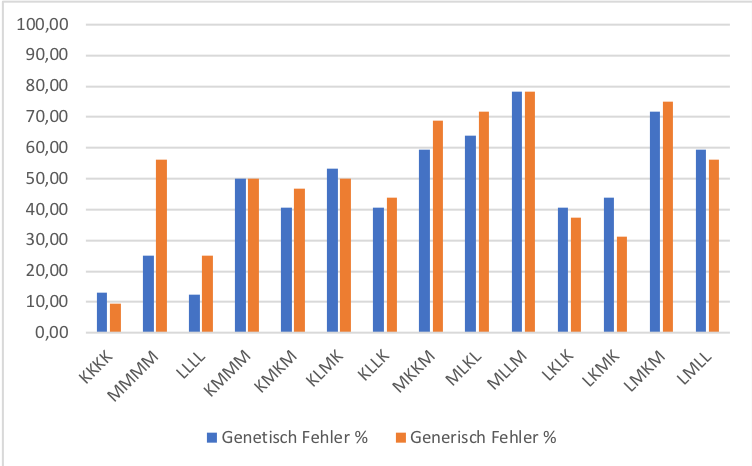
\includegraphics[width=\textwidth]{pics/analyse/algo/ohneFehler/Fehler4.png}
	\end{minipage}
	\begin{minipage}[t]{0.4\textwidth}
		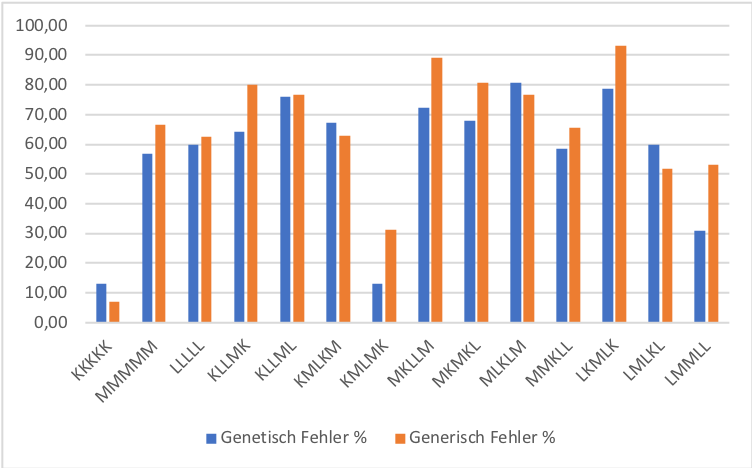
\includegraphics[width=\textwidth]{pics/analyse/algo/ohneFehler/Fehler5.png}
	\end{minipage}
	\caption{Anhand der Diagramme wird die H{\"a}ufigkeit, wie oft einem Muster nicht richtig erkannt worden ist. Es z{\"a}hlt ein Muster als nicht erkannt, wenn mindestens ein Signal nicht korrekt zugrordnet werden konnte.   
	%Darstellung der Wahrscheinlichkeit {\"u}ber alle Probanden, wie oft bei einem Muster mindestens ein Signal nicht korrekt zugeordnet werden konnte.
	Dabei wurden die genetischen und generischen Fehlerangaben (in \%) direkt miteinander verglichen. 
	Die Diagramme wurden f{\"u}r die jeweiligen Muster (dreier, vierer und f{\"u}nfer) seperat angezeigt.
	Hier steht K f{\"u}r \textit{Kurz}, M f{\"u}r \textit{Mittel} und L f{\"u}r \textit{Lang}}
	\label{fig:FehlerBild}
\end{figure}
 
In der Darstellung \autoref{fig:FehlerBild} wurden die Muster und die H{\"a}ufigkeit, wie oft die Probanden das Muster nicht als solches erkannt haben, dargestellt. 
Die Muster \textit{KKK} und \textit{LLL} haben die meisten Probanden korrekt erkannt, nur 12 \% haben bei den genetischen Werten das Signal nicht korrekt erkennen k{\"o}nnen. 
Au{\ss}erdem wurden hat man bei den selben Mustern mit den generischen Werten eine Verschlechterung von 7\% bei \textit{KKK} und eine Verdopplung bei \textit{LLL} festgestellt, wobei man das gleiche Verhalten auch bei den vierer Muster erkennen kann.

Im Vergleich der drei Diagramme kann man erkennen, dass f{\"u}r die dreier und vierer Muster mit nur einem Signaltypen bei \textit{Kurz} und \textit{Lang} nahezu identisch sind und die genetischen Muster {\"o}fter erkannt wurden als die generischen Muster. 
Das Muster mit durchgehenden \textit{Mittel} Signalen haben die Probanden bei den dreier sowie bei den vierer Mustern jeweils das genetische bevorzugt, da die generischen Muster um jeweils das Doppelte schlechter erkannt wurde. 

Unter allen dreier Mustern wurden zwei drittel der genetischen Muster besser als die generischen Muster erkannt. 
Zus{\"a}tzlich befindet sich der Durschnitt bei 36\% f{\"u}r die genetischen und bei 43\% f{\"u}r die generischen dreier Muster.
Dieser Prozenzssatz steigt bei den genetischen vierer Muster auf 46\% und bei den gernerischen auf 50\%, bei den f{\"u}nfer ist der Wert bei 57\% f{\"u}r die genetischen und bei 64\% f{\"u}r die generischen Muster. 
Anhand dieser Daten kann man sagen, je h{\"o}her die Anzahl der Signale in einem Muster werden, desto weniger Probanden k{\"o}nnen diesen noch richtig erkennen.

Desweiteren kann man feststellen, dass die genetischen vierer Muster nur noch eine minimale Abweichung zu den generischen Muster aufweisen, das selbe ist auch bei den f{\"u}nfer Mustern zu erkennen.
Vor allem habe sich im durch dem erh{\"o}hen nicht alles verschlechtert, denn bei dem auf- und wieder absteigenden Muster \textit{KMLMK} haben die Probanden es genauso gut erkannt, wie das durchg{\"a}ngige Kurze f{\"u}nfer Muster. 

Die meisten Probanden haben bei den Mustern nur ein Signal falsch erkannt oder haben es um eine Signaltypen h{\"o}her oder niedriger bewertet, dabei  haben die aber dennoch erkannt, dass die Signale sich ver{\"a}ndert haben. Als Beispiel haben Sie das Muster \textit{LMMLL} als \textit{MKKMM} bewertet. \\

\begin{figure}[htbp] 
            \centering
   	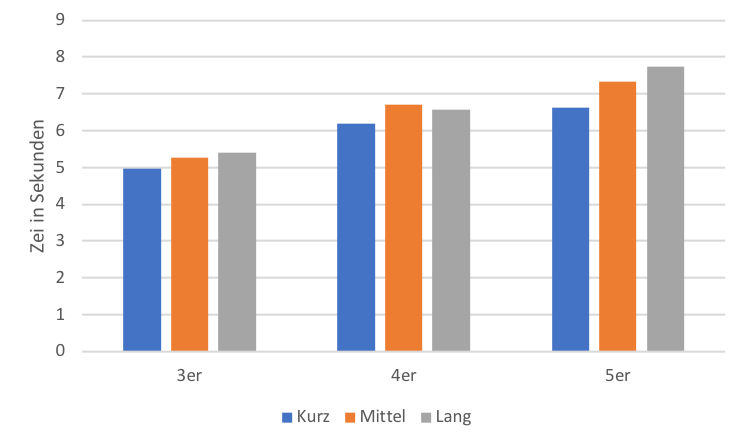
\includegraphics[width=\textwidth]{pics/analyse/algo/ZeitbenoetigtSignalMuster.png}
	\caption{Durchschnittlich ben{\"o}tigte Zeit der Probanden, um ein Signal eines Musters zu erkennen}
	\label{fig:ZeitbenoetigtSignalMuster}
\end{figure}
Im Gegensatz zu der ben{\"o}tigten Zeit beim Algorithmus \autoref{fig:ZeitDurchschnitt}, hat man f{\"u}r jeden Muster-Typen der ein weiteres Signal hinzugef{\"u}gt hat, mehr Zeit ben{\"o}tigt um ein Signal zu erkennen \autoref{fig:ZeitbenoetigtSignalMuster}. 
Die Zeiten f{\"u}r die Muster mit drei Signalen haben sogar eine bessere Zeit als die letzte Iteration vom Algorithmus. 
Alle Signaltypen bei dem dreier Muster haben eine {\"a}hnliche Durchschnittliche Erkennungszeit von f{\"u}nf Sekunden.
%Im Vergleich der Signaltypen bei den dreier Muster-Typen untereinander, wurden unter den dreier Signaltypen jeweils eine Durschnittliche Zeit von ca f{\"u}nf Sekunden ben{\"o}tigt.
Man kann gut erkennen, wie bei den vierer und f{\"u}nfer Muster jeweils die Signaltypen um eine Sekunde mehr Zeit ben{\"o}tigen um diese zu erkennnen, als die dreier Muster.

\begin{table}[]
\centering
\caption{anova}
\label{Erkennungsrate (und Standardabweichung) der Mustertypen. Dabei wurden die Genetischen und Generischen Signale miteinander vergliechen}
\begin{tabular}{l|ll}
              & Genetisch     & Generisch     \\ \hline
3 Vibrationen & 0,817 (0,135) & 0,786 (0,106) \\
4 Vibrationen & 0,771 (0,148) & 0,729 (0,147) \\
5 Vibrationen & 0,756 (0,123) & 0,686 (0,138)
\end{tabular}
\end{table}

Mittels einer Varianzanalyse habe man die Werte aus der \autoref{anova} bestimmt. 
Es hat sich ergeben, dass die Probanden signifikant schlechter abgeschnitten sind, als man sie mit einem komplexeren Mustern konfrontiert hat, im Vergleich zu weniger komplexeren Mustern. 
Eine weitere Erkentniss ist gewesen, dass die genetischen Muster besser erkannt wurden als die generischen Muster.

















%% ==============================
%\section{Zusammenfassung}
%% ==============================
%\label{ch:Evaluierung:sec:zusammenfassung}


%%% Local Variables: 
%%% mode: latex
%%% TeX-master: "diplarb"
%%% End: 


%% zusammenf.tex
%% $Id: zusammenf.tex 4 2005-10-10 20:51:21Z bless $
%%

\chapter{Zusammenfassung und Ausblick}
\label{ch:Zusammenfassung}
%% ==============================
Bla fasel\ldots

(Keine Untergliederung mehr!)

%%% Local Variables: 
%%% mode: latex
%%% TeX-master: "diplarb"
%%% End: 



GLOSSAR

Force Feedback:




\paragraph{Auswertung}
Man kann feststellen, das je mehr Signale man in ein Muster packt, desto höher wird die Wahrscheinlichkeit, dass die Muster nicht korrekt erkannt werden. 

Die Probanden haben niemals eine Rückmeldung darüber erhalten, ob Sie richtig oder falsch liefen.

%% zusammenf.tex
%% $Id: zusammenf.tex 4 2005-10-10 20:51:21Z bless $
%%

\chapter{Zusammenfassung und Ausblick}
\label{ch:Zusammenfassung}
%% ==============================
Bla fasel\ldots

(Keine Untergliederung mehr!)

%%% Local Variables: 
%%% mode: latex
%%% TeX-master: "diplarb"
%%% End: 





%% --------------------
%% |   Bibliography   |
%% --------------------
\cleardoublepage
\phantomsection
\addcontentsline{toc}{chapter}{\bibname}

\iflanguage{english}
{\bibliographystyle{IEEEtranSA}}	% english style
{\bibliographystyle{babalpha-fl}}	% german style
												  
% Use IEEEtran for numeric references
%\bibliographystyle{IEEEtranSA})

\bibliography{ausarbeitung}
\Erklaerung
\end{document}
